%!TEX root = ../thesis.tex
%*******************************************************************************
%****************************** Third Chapter **********************************
%*******************************************************************************
\chapter{Developing a method to integrate and classify cell types across tissues} \label{chap:CT_method}

% **************************** Define Graphics Path **************************
\ifpdf
    \graphicspath{{Chapter3/Figs/Raster/}{Chapter3/Figs/PDF/}{Chapter3/Figs/}}
\else
    \graphicspath{{Chapter3/Figs/Vector/}{Chapter3/Figs/}}
\fi
The widespread adoption of single-cell sequencing technologies has revolutionised the molecular profiling of cells. The use of these methods allows us to understand the building blocks of tissues at an unprecedented resolution. As further human tissues are examined, a catalog of cell types and their gene expression profile can be compiled from published data. 

This chapter outlines the development of a computational pipeline for cross-tissue integration of scRNA-seq data, illustrating the performance of individual steps in a controlled dataset. The pipeline is tuned to capture cell type similarities from annotated and non-annotated data between tissues, resulting in an unbiased gene expression reference for cell type identity. This reference can then be used to train \textit{CellTypist}, a set of logistic regression classifiers capable of assigning cell type identity to newly produced scRNA-seq data. \textit{CellTypist} is trained on the \textit{Tabula Muris} dataset as a mouse reference, and on a large collection of tissue-derived human data.

This project was initially conceived together with Valentine Svensson while he was part of the Teichmann group. The human data collection and integration was performed with the assistance of Ni Huang. The mouse and human cell type references trained here are further analysed in Chapter~\ref{chap:CT_test}.


\section{Introduction}
\label{section3.1}
The growth of the scRNA-seq field is in part due to an increasing number of complex and detailed cellular census of individual tissues, often directly associated with large consortia that aggregate these datasets and establish guidelines and collaborations to identify all cell types across an organism~\citep{regev_human_2017}. Individually, these studies have provided crucial insights into cell biology. Nonetheless, the data generated can often be reused for new purposes, either on its own to extract new conclusions, or through combination or comparison with novel data. 

% integration methods, classification methods, comparison
To combine scRNA-seq datasets, batch correction and batch alignment methods seek to either correct gene expression values accounting for technical metadata~\citep{ritchie_limma_2015,johnson_adjusting_2007,buettner_f-sclvm:_2017,haghverdi_batch_2018,buttner_test_2019}, or place cells from different batches, technologies and datasets in a common manifold, allowing joint clustering and pseudotime analysis~\citep{butler_integrating_2018,polanski_bbknn:_2019,hie_efficient_2019,korsunsky_fast_2018,stuart_comprehensive_2019}. Conversely, comparison between scRNA-seq datasets aims to impart the knowledge gained from one dataset into another, usually through classification models. Various methods have been developed to compare cell types (and indeed other labels) across datasets (reviewed in Chapter~\ref{section1.3}, Table~\ref{table:tab_1_2}). A benchmark of 22 classification methods for scRNA-seq~\citep{abdelaal_comparison_2019} has revealed SVM-based classifiers as the top performing ones, capable of accurate cross-dataset classification and handling of all genes by using L2 regularisation. This study also echoed the findings of another recent study~\citep{kohler_deep_2019} that demonstrated that deep learning methods do not outperform classical machine learning approaches, including SVM and logistic regression, for cell type classification.

% short description of the chapter
%% mention nomenclature: cell types - prior annotation; clusters - any derived, not named labelling. CellTypist, by default, uses CLUSTERS
Despite the high accuracy of there tools, which are highly effective at annotating new data using specific datasets, their scope will is limited to the dataset chosen as a reference and don't directly handle large collections of data. To address the need for a reference that can allow fast and automatic annotation across tissues, we have developed a pipeline for integration of scRNA-seq data obtained from a variety of tissues, which can then be used to build \textit{CellTypist}, a global cell type classification method based on logistic regression classifiers. While previous work has been developed for well annotated mouse data using a neural network-based classifier~\citep{alavi_web_2018}, \textit{CellTypist} can leverage data with different annotations, focusing on providing broad identifiers for cells based on a reference from pooled data. 

This chapter discusses the structure of the integration and classification pipeline, exploring its strengths and caveats, with each step performed on the \textit{Tabula Muris} data~\citep{noauthor_single-cell_2018}. Despite coming from a sole publication, this dataset has the advantage that it was generated in highly controlled conditions, spans 20 tissues, and includes a detailed and robust cell type annotation to be used as a ground truth for the performance of each stage. The methodology outline is then used to train classifiers based on the \textit{Tabula Muris}, as well as a collection of human data of close to 1.5 million cells. The training accuracy and bias of the models is assessed and discussed, with suggestions for further improvements.

\textit{CellTypist} is further explored in Chapter~\ref{chap:CT_test}, where its application will be tested for automatic classification. It will also be explored in terms of biological insights, in order to identify cross-tissue relationships and examine which genes the model deemed important to determine cell identity.


\nomenclature[z-SS2]{SS2}{Smart-seq2}

\section{Methodology}
\label{section3.2}
\subsection{Per-tissue clustering to approximate cell type annotations}
\label{section3.2.1}
Processing the data that will be used as a reference in \textit{CellTypist} follows three major steps. First, the data collected follows a procedure for uniform per-tissue processing (Figure~\ref{fig:chap3_pertiss}A). Next, the clusters determined in each tissue are matched across the whole dataset (Figure~\ref{fig:chap3_combcl}A). Lastly, the combined clusters are used as labels to train a logistic regression classifier using the complete data collection (Figure~\ref{fig:chap3_model}A).

Most scRNA-seq studies profile cellular heterogeneity in one specific biological sample, which often results in reporting the cell types or cell states present. While this is clearly displayed in the figures from these studies, this information in not always supplied in a machine-readable format, associated with either the raw sequencing reads or the quantified gene expression. Furthermore, most annotations do not follow a uniform, controlled vocabulary~\citep{bard_ontology_2005}, and is often done at varying resolutions depending on the focus of the study or the breadth of the dataset.

The pipeline starts by splitting the collected data by tissues, grouping together data from different studies that profile the same body part, even if using distinct scRNA-seq protocols (Figure~\ref{fig:chap3_pertiss}A). At this stage, data from each tissue is processed following a uniform workflow using scanpy~\citep{wolf_scanpy:_2018}. Gene expression is normalised by their total counts and log transformed, and different datasets are batch aligned using BBKNN~\citep{polanski_bbknn:_2019}. Lastly, clustering at varying resolutions using the Leiden algorithm~\citep{traag_louvain_2019} is performed. This processing is executed to ensure that all tissues are similarly treated, regardless of the level of annotation, and to allow unannotated data to be included and bolster \textit{CellTypist}'s training data.

\begin{figure}[pht!]
    \centering    
    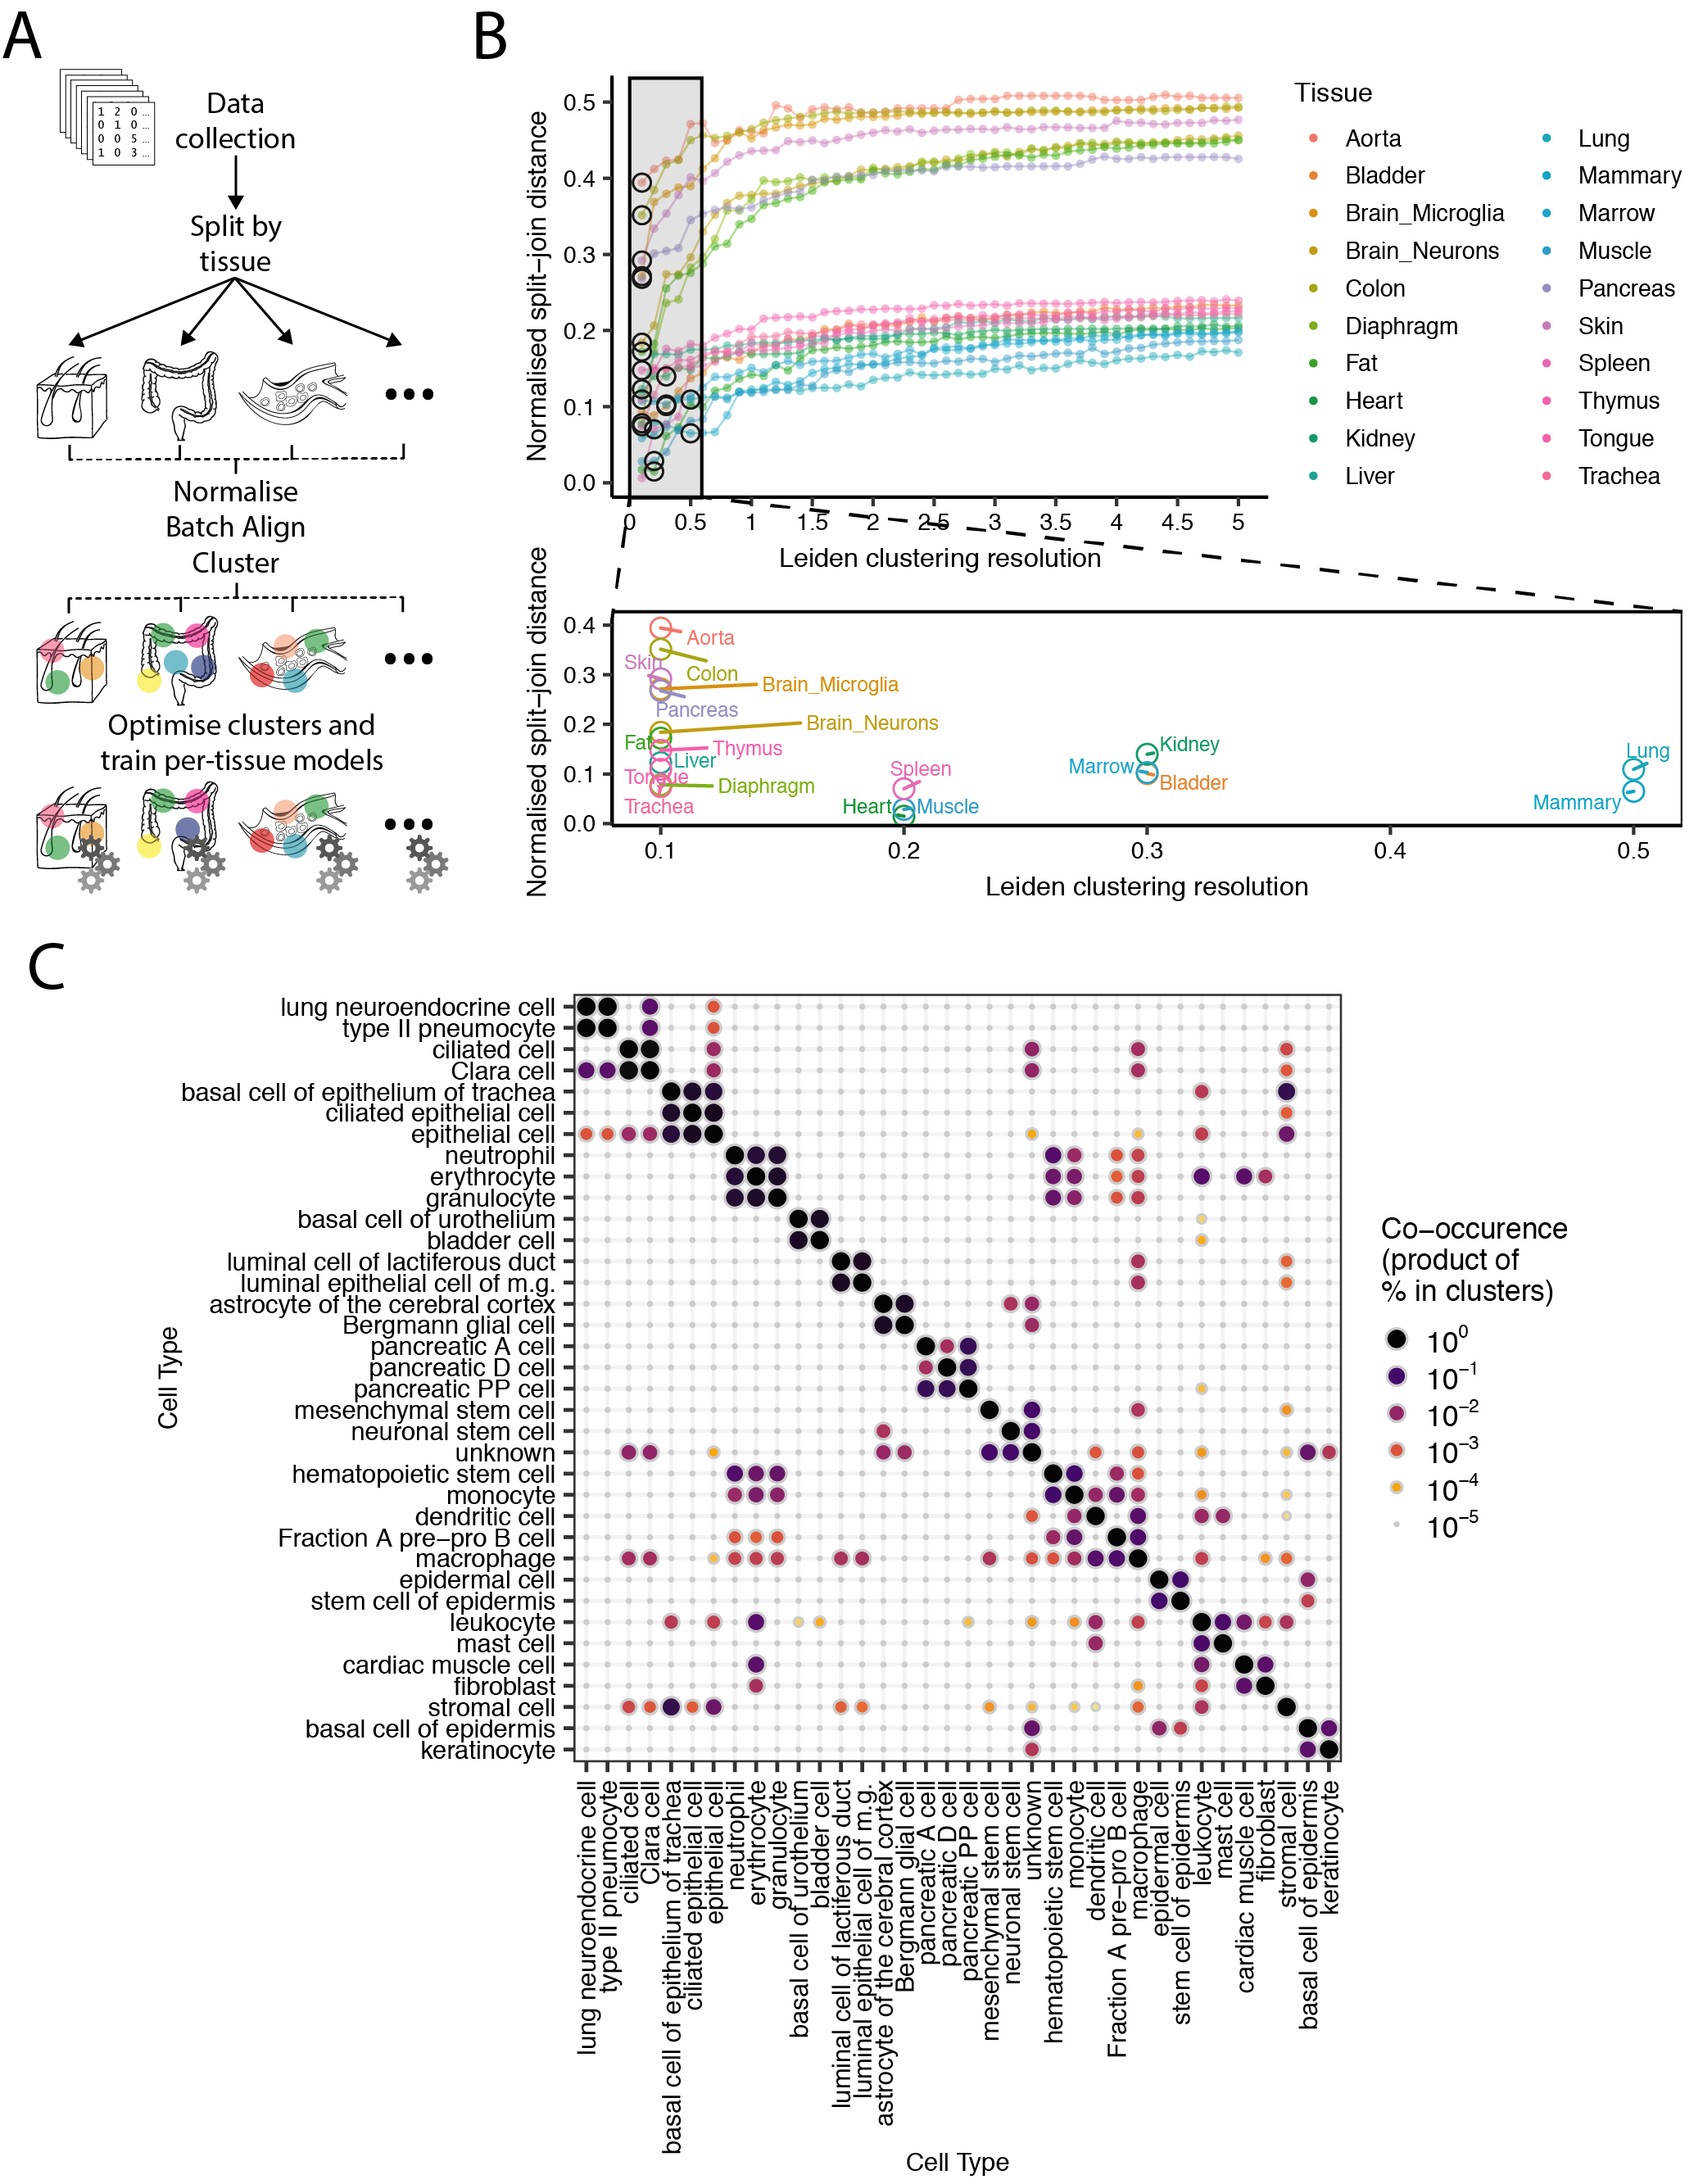
\includegraphics[width=1.0\textwidth]{Chapter3/Figs/chap3_TMperTissue.png} % change word in curlies to change figure
    \caption[Data reprocessing per-tissue]{\textbf{Data reprocessing per-tissue}\newline\textbf{(A)} Pipeline for initial data processing. Data collected is split into tissue, followed by integration of different datasets (in \textit{Tabula Muris}, different protocols), and clustered to optimally match existing cell type annotations. (Continued on the following page.)}
    \label{fig:chap3_pertiss}
\end{figure}
\begin{figure}[t]
  \contcaption{(continued) \textbf{(B)} Per-tissue cluster optimisation, choosing the resolution that approximates existing cell type annotations. Similarity is measured with normalised split-join distance, and constrained to solutions with a number of clusters of at least as many as existing annotations in the tissue. Upper panel shows the full range of resolutions tested per-tissue; lower panel shows the resolution range in which the optimal value for each tissue was present. \textbf{(C)} Co-occurrence of annotated cell types in the same clusters, determined by summing the products of each cell types per-cluster percentage. Only cell types with at least one co-occurrence value of 0.05 were kept. m.g. - mammary gland.}% Continued caption
\end{figure}

% explain SJ
The clustering performed in each tissue can be optimised to approximate existing cell type labels. To this end, various groupings were generated in each tissue using a range of values for the resolution parameter of the Leiden algorithm. The clusters obtained were subsequently compared to known cell type annotations. The distance between clusters and cell types was calculated using the normalised split-join (SJ) distance~\citep{dongen_performance_2000}. Briefly, SJ distance measures the distance between two data partitions according to the number of element-wise division (split) or merge (join) operations necessary to fully convert the new partition into the former. In this specific example, it counts the number of operations necessary to convert the new clustering groups back into any known cell type annotations. Since the values in the original metric are dependent on the number of elements being cluster, and which here differ between tissues, Figure~\ref{fig:chap3_pertiss}B shows a normalised version of the metric, where it was divided by 2N, with N = number of cells for a given tissue. Its values will fall in an interval between 0 and 1, corresponding to complete similarity or complete dissimilarity. 

The calculated normalised SJ distance for each Leiden clustering resolution tested is plotted in Figure~\ref{fig:chap3_pertiss}B (top). The chosen resolutions (black circles) are a result of Leiden clustering that 1) outputs at least as many clusters as there are unique cell type labels in the largest dataset contributing to that tissue, and 2) has the lowest normalised split-join distance. Despite the broad range of clustering resolutions tested, (from 0.1 to 5 at 0.1 intervals), the parameters chosen for all tissues concentrated at resolutions of up to 0.5 (Figure~\ref{fig:chap3_pertiss}B, top shaded box and bottom expansion). Tissues appeared to organise into two distinct groups: a smaller group with an SJ distance above 0.2, and a larger one with a distance below 0.2. Interestingly, all tissues in the higher SJ distance group were only sequenced using Smart-seq2 (Figure~\ref{fig:appB_tmcounts}), suggesting that integration of data from different protocols is not resulting in clusters that incorrectly approximate known cell types. This group also had, in general, fewer cell types annotated, thus the higher values could be explained by overclustering.

To understand the extent of misclustering of cell types within the per-tissue clustering step, co-clustering of known cell types was examined across all tissues (Figure~\ref{fig:chap3_pertiss}C). We started with a cell type-by-cluster matrix, showing the distribution of cell types per cluster as a percentage. To obtain a symmetric matrix, i.e. show the co-occurrence of two cell types normalised for the occurrence of each cell type, we obtained the product of this matrix with its transposed form. The resulting matrix is subsequently filtered to only include cell types with at least one co-occurrence value of 0.05 (meaning more than 20\% of the cells from each cell type in a pair would appear in the same clusters). Besides a high clustering of cells with the same annotation, the plot shows that most of the mixing happens between related cell types (e.g. epithelial cell, ciliated epithelial cell and basal cell of epithelium of trachea; luminal cell of lactiferous duct and luminal epithelial cell of mammary gland), or between hematopoietic-derived cells (e.g. neutrophil, erythrocyte, granulocyte; hematopoietic stem cell, macrophage and dendritic cell; leukocyte and mast cell). This is expected due to the similarities between related cell types, as well as due to less resolved clustering of immune and non-immune cells when these are analysed together. Another possible explanation is the existence of doublets, yet these tend to happen between specific pairs of cell types, which was not the most common case.

Overall, despite some losses in the resolution of cell groupings, the per-tissue clustering step of \textit{CellTypist} maintains much of the cell type information existing in the original data.


\nomenclature[z-SJ]{SJ}{split-join (distance)}

\subsection{Combining cell clusters across tissues using tissue-specific classifiers}
\label{section3.2.2}
In order to obtain a global reference for cell type classification, cell identity should be harmonised between all surveyed tissues. To achieve this, the clusters obtained at the end of the previous step are used as target labels predicted from gene expression using logistic regression models for each tissue (Figure~\ref{fig:chap3_combcl}A, left). Model characteristics and training parameters are detailed in Section~\ref{section3.2.3}. These models are then used to classify the complete datasets, thus obtaining assignment probabilities to the clusters in every tissue for each cell. These probabilities are further averaged per cluster, so that we obtain a mean probability of every per-tissue cluster corresponding to all others.

\begin{figure}[pht!]
    \centering    
    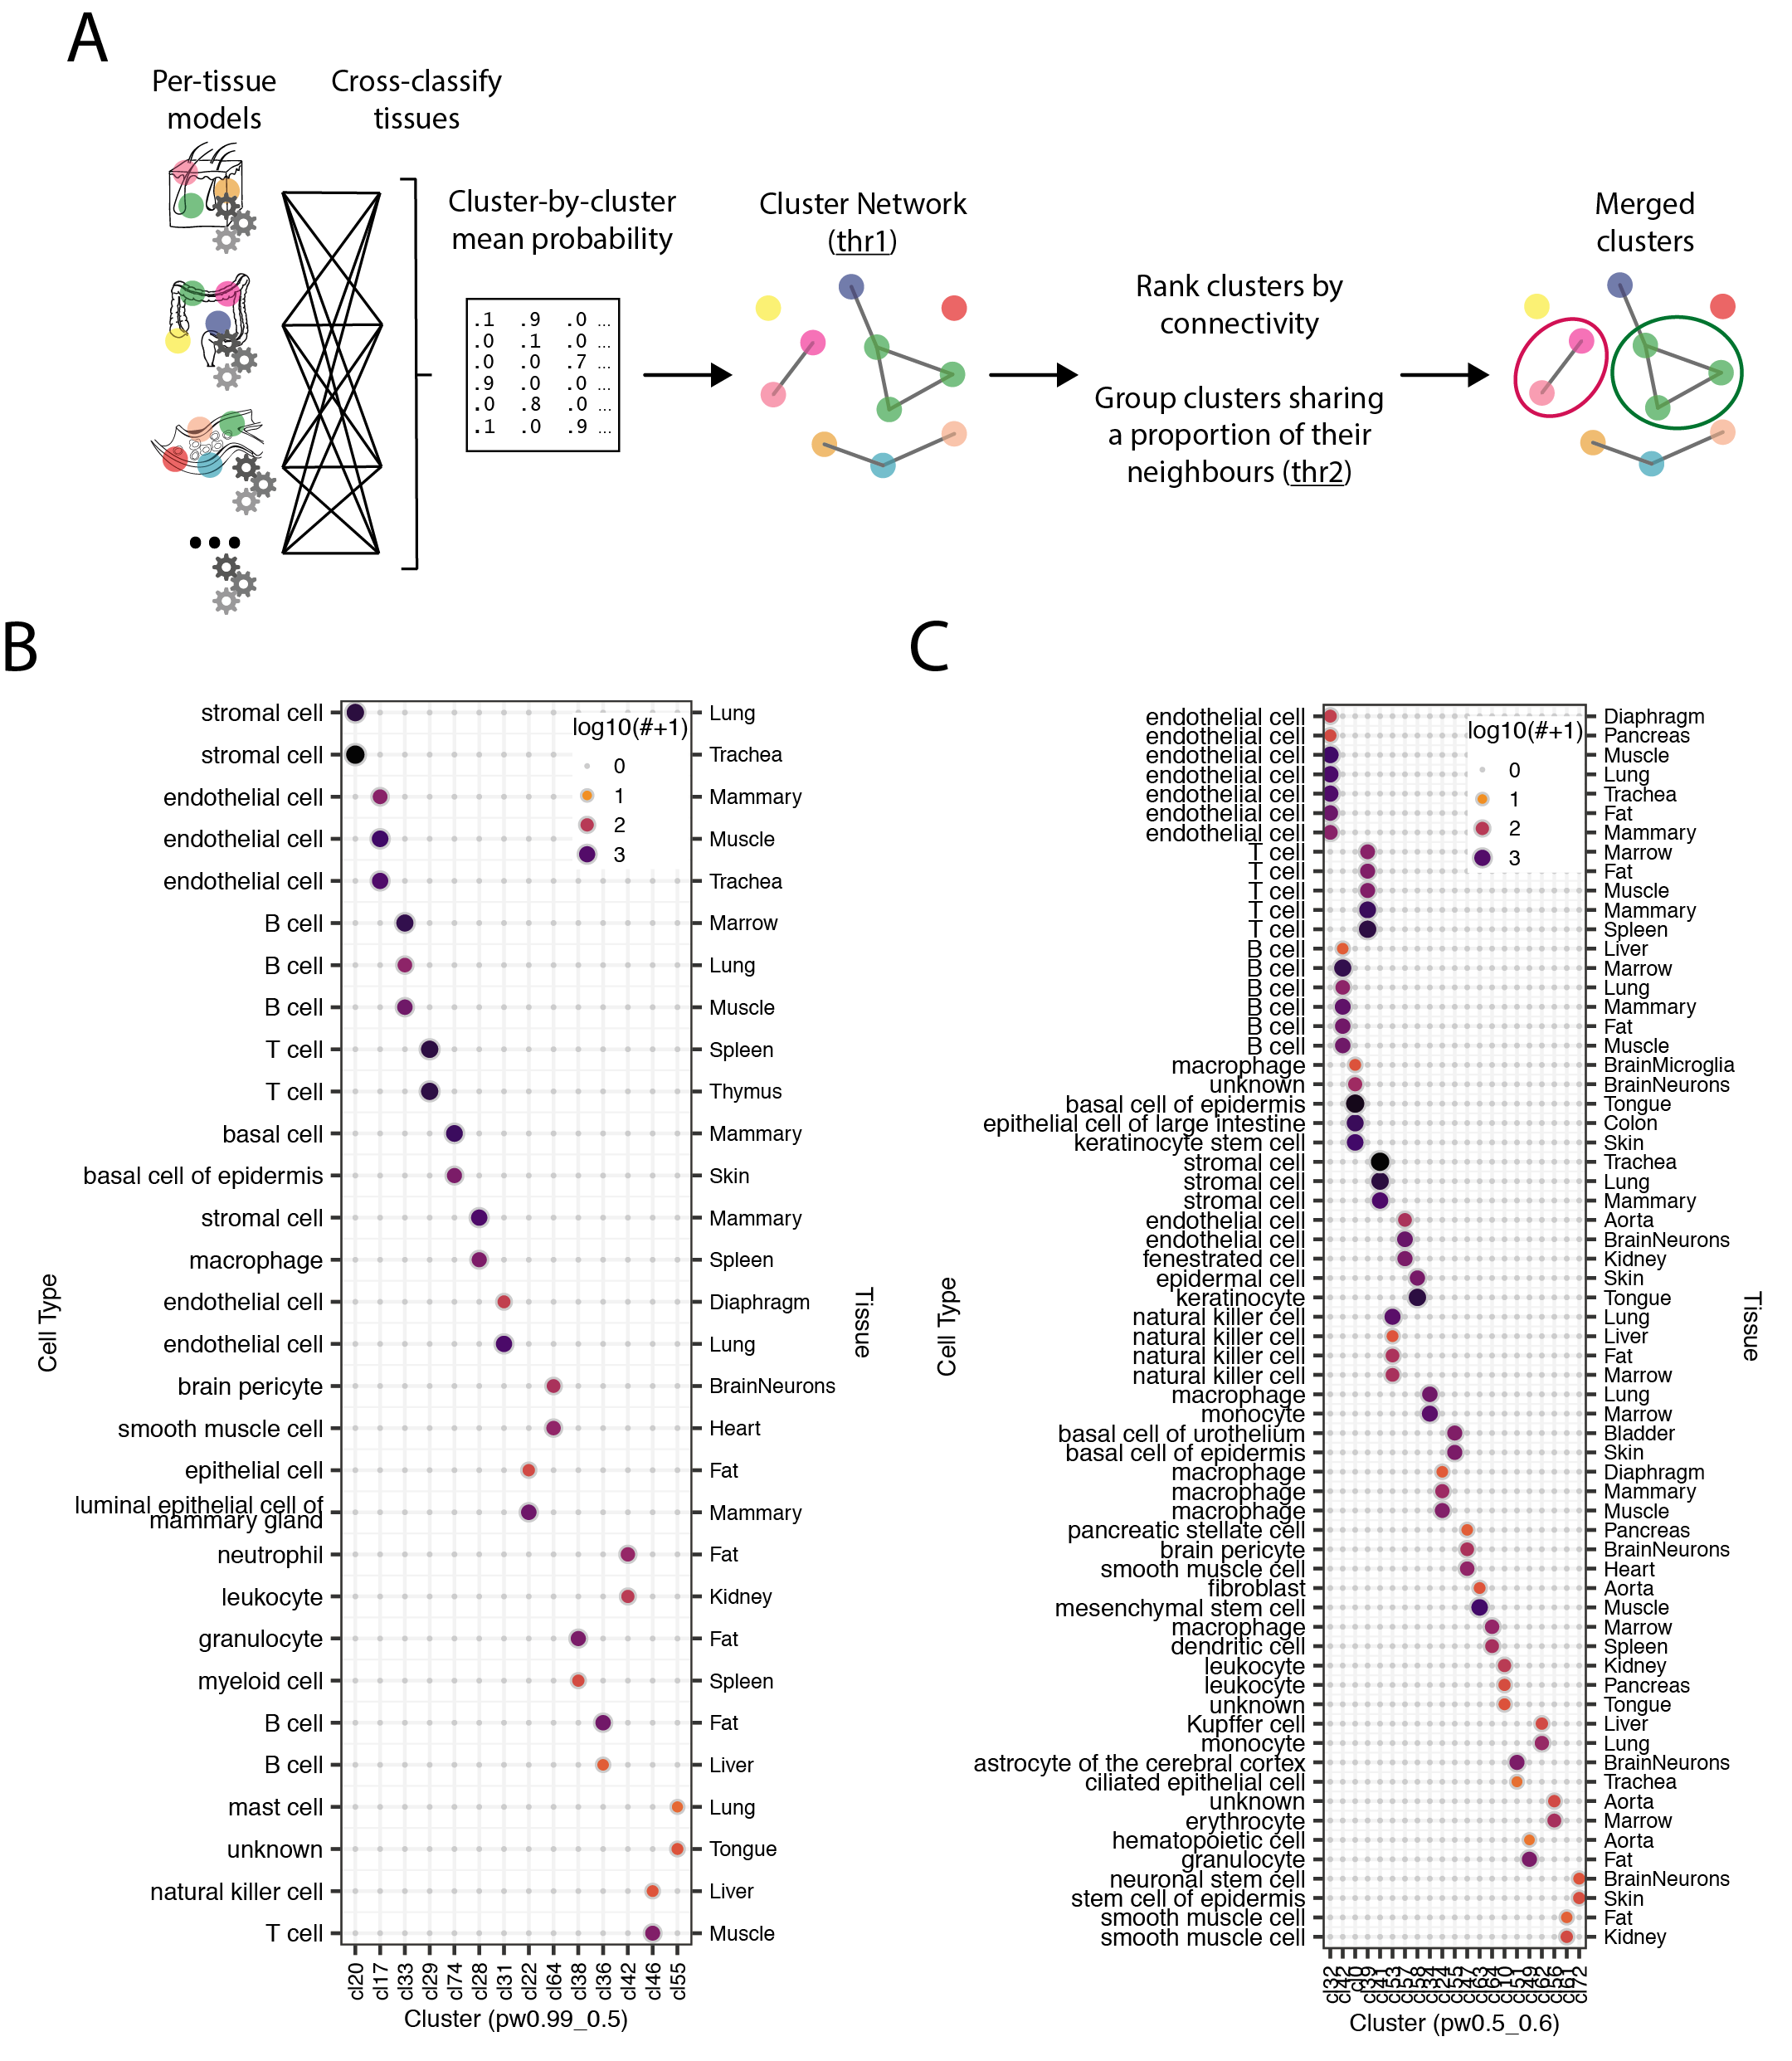
\includegraphics[width=1.0\textwidth]{Chapter3/Figs/chap3_combineClusters.png} % change word in curlies to change figure
    \caption[Cross-tissue matching of cell types]{\textbf{Cross-tissue matching of cell types}\newline\textbf{(A)} For each tissue, a logistic regression model is trained, and used obtain a classification probability of all tissues. Clusters are then linked depending on the mean probabilities of one cluster matching another (\textit{thr1}). Clusters are ranked on connectivity, and grouped with neighbouring clusters that share a proportion of its neighbours (\textit{thr2}). (Continued on the following page.)}
    \label{fig:chap3_combcl}
\end{figure}
\begin{figure}[t]
  \contcaption{(continued) \textbf{(B and C)} Merging of cell types (x-axis) using the method in (A) for models trained on known cell type labels (left y-axis). \textbf{(B)} shows the top parameter combination (thr1 = 0.99, thr2 = 0.5) based on split-join distance; \textbf{(C)} shows the combination that came in third (thr1 = 0.5, thr2 = 0.6) and which resulted in increased merging.}% Continued caption
\end{figure}

% explain thresholds/algorithm
The merging of clusters is dependent on two parameters. The first (thr1) is defined as a threshold for the dot product of the mean probabilities of two clusters, above which they are considered similar (i.e. "connected"). Based on this we can obtain a network with the connections between all clusters (Figure~\ref{fig:chap3_combcl}A, middle). This network serves as the base to define the cluster groupings. Clusters are then ranked based on their degree (i.e. the number of clusters they connect to) and grouped with their neighbours that share at least a defined percentage of their neighbours (thr2) (Figure~\ref{fig:chap3_combcl}A, right). The clusters merged are removed from the ranking, and the condition is iteratively applied until it has been tested for all elements. Lastly, the solutions for all thresholds are ranked based on their improvement over the per-tissue labels as measured by the split-join distance (detailed below).

% B and C - testing using the cell types as labels - what cell types get merged?
To assess how this algorithm performed in a situation with known labels, it was tested using the annotated cell types for each tissue instead of clusters. After ranking the solutions given by the different parameter combinations tested (combinations identical to Figure~\ref{fig:chap3_combdat}B), we inspected the top parameter combination (Figure~\ref{fig:chap3_combcl}B, thr1 = 0.99 and thr2 = 0.5), as well as the third, which presented the lowest combined cluster number (Figure~\ref{fig:chap3_combcl}C, thr1 = 0.5 and thr2 = 0.6). Most clusters resulting from the merging workflow, in both solutions, combined cell types annotated with the same name in different tissues. This is particularly evident for endothelial cells, B cells, and T cells. While the score for the merging  presented in panel C was not as good as that for panel B, it is immediately apparent that the more extensive merging still conserves most of the correct labeling, even grouping together identical cell types that are left separate in the first solution. This indicates that there can be a range of approximately correct parameter combinations, and hints at the tissue specificity of certain widespread cell types. Taking as an example endothelial cells, the first combination leaves lung and diaphragm separate from the remaining tissues.

\begin{figure}[hb!]
    \centering    
    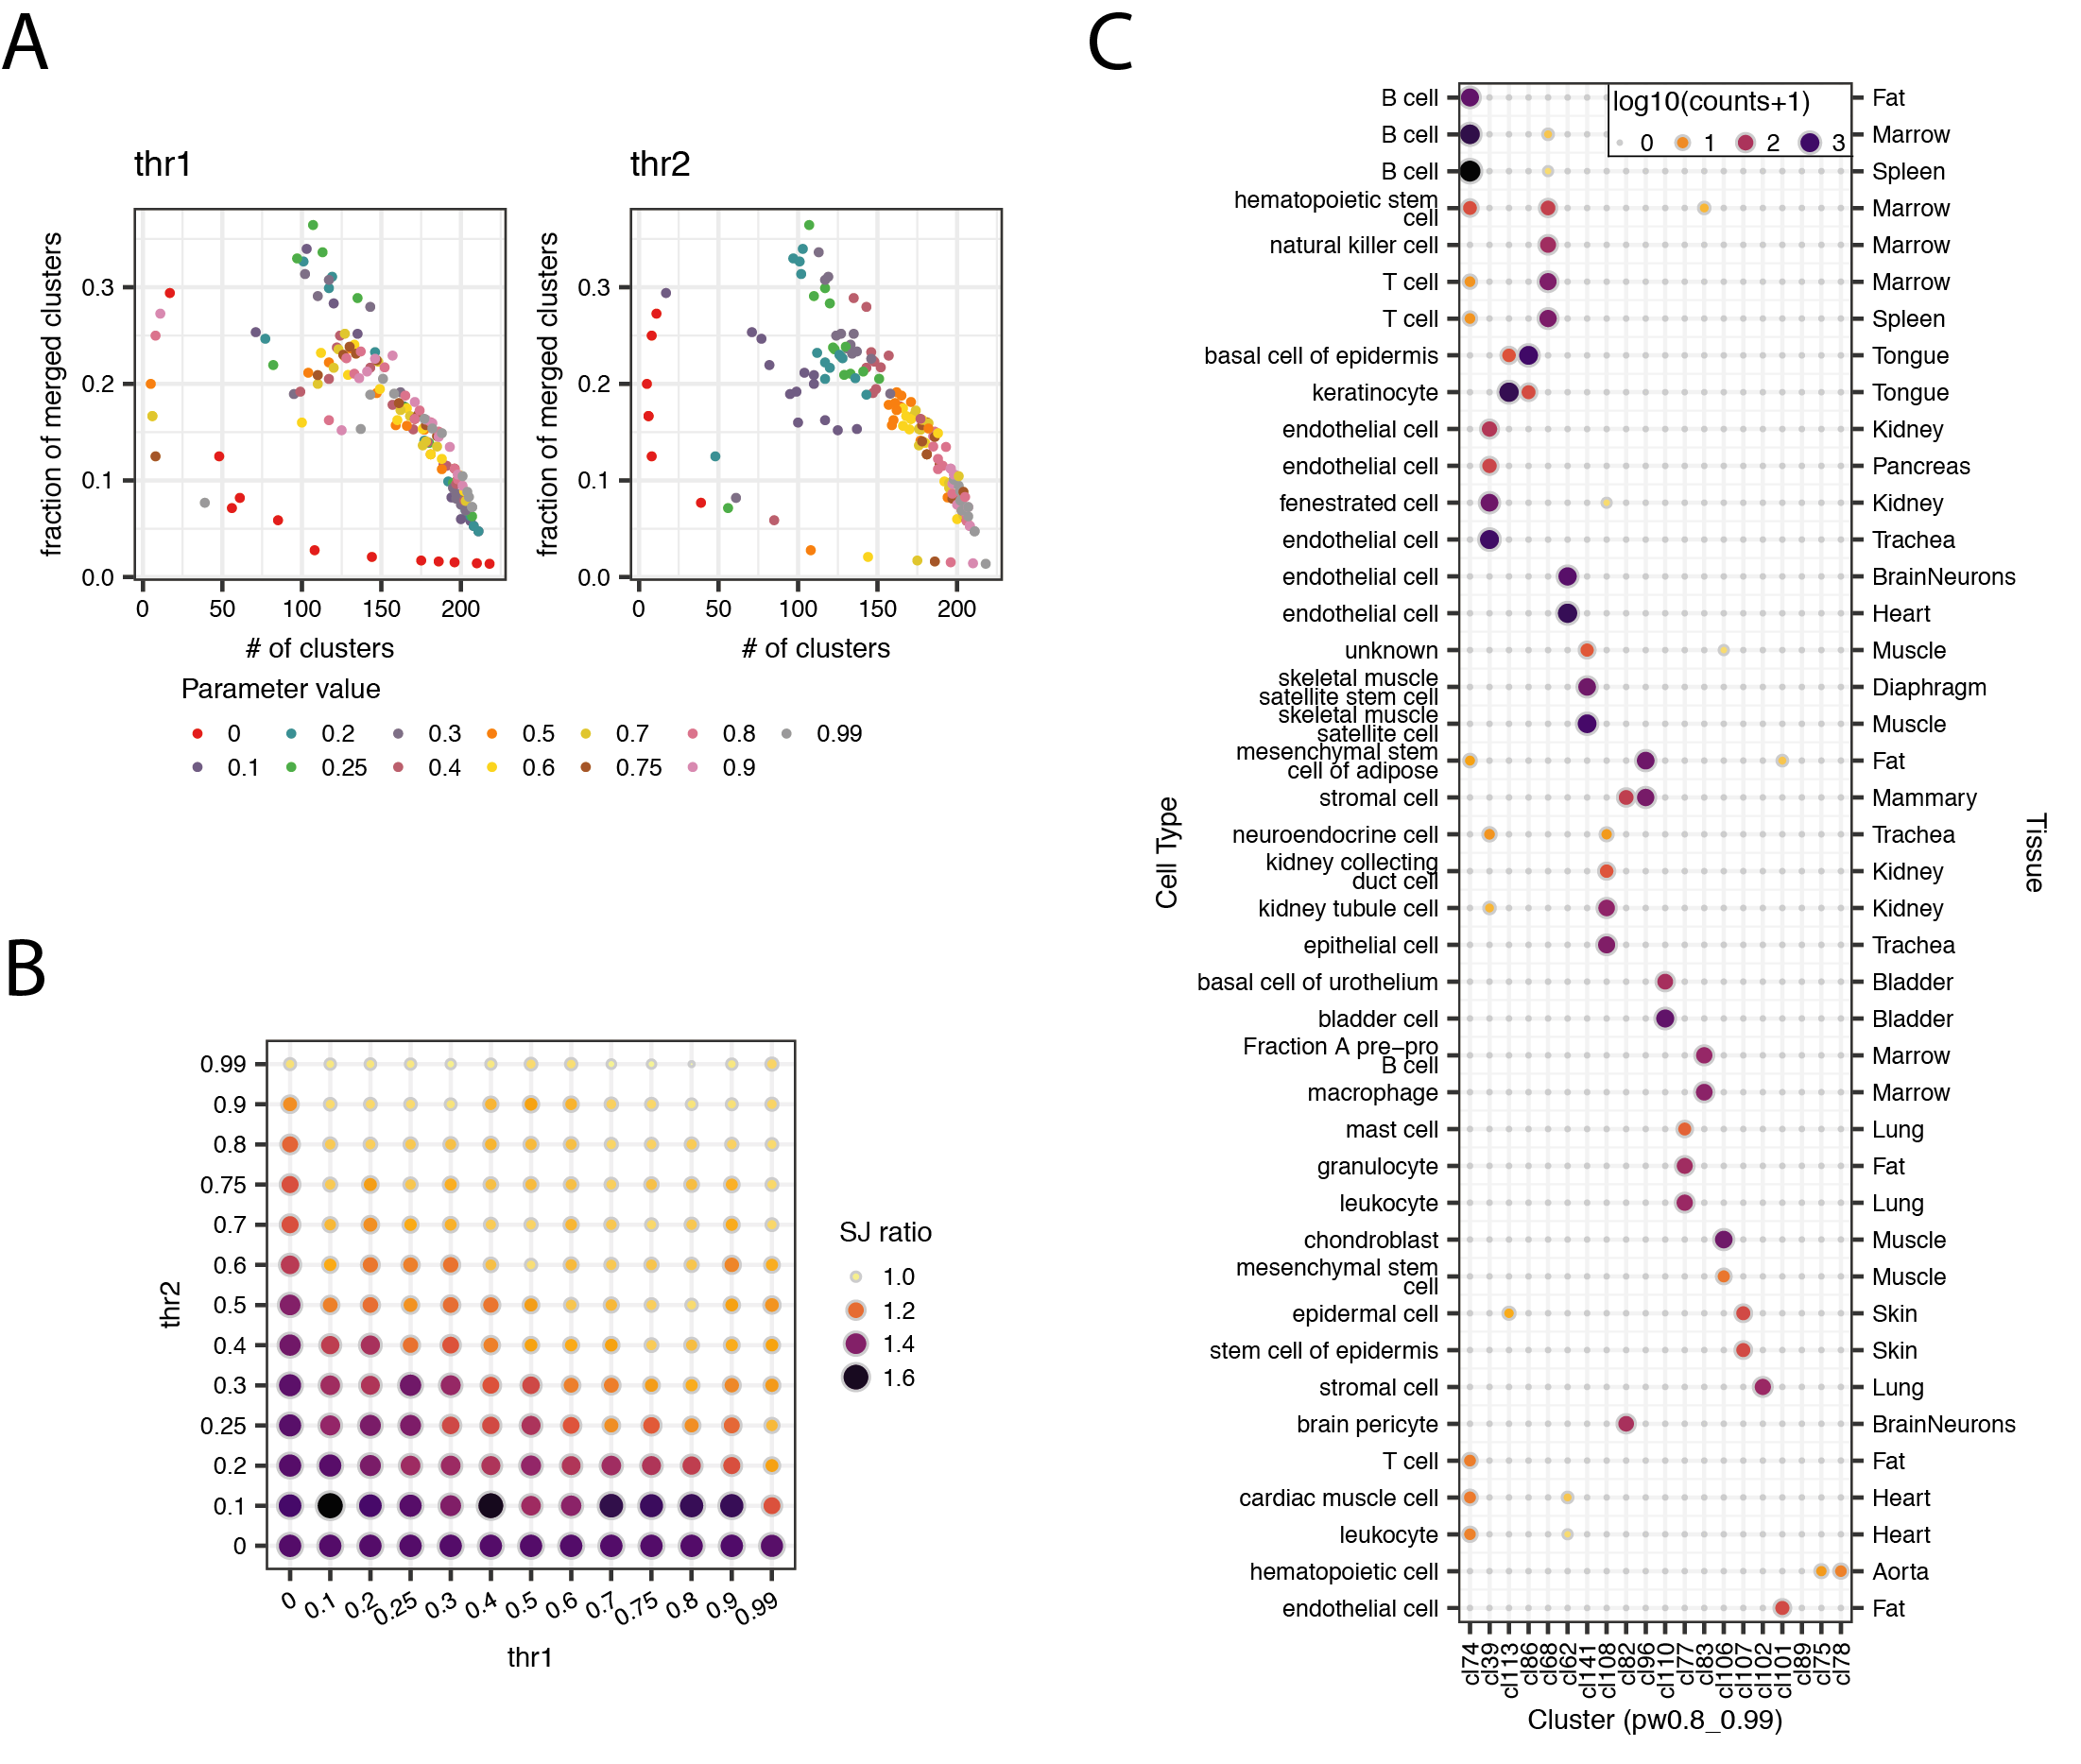
\includegraphics[width=1.0\textwidth]{Chapter3/Figs/chap3_combineData.png} % change word in curlies to change figure
    \caption[Evaluation of clusters matched across tissues]{\textbf{Evaluation of clusters matched across tissues}\newline\textbf{(A)} Change in number of total clusters and fraction of merged clusters with each threshold value (see Figure~\ref{fig:chap3_combcl}A for reference). Parameters resulting in a single cluster were not represented. \textbf{(B)} Parameter grid showing the variation of the ratio of split-join distance between merged clusters and cell type annotation, and per-tissue clusters and cell type annotation. \textbf{(C)} Grouping of cell types contained in per-tissue clusters (x-axis) using the top parameter combination (thr1 = 0.8, thr2 = 0.99) based on split-join distance.}
    \label{fig:chap3_combdat}
\end{figure}

% how it looks with clusters
This merging was then performed on the tissue clusters obtained from the first section of the pipeline. Both thresholds in the algorithm were tested with the values 0, 0.1, 0.2, 0.25, 0.3, 0.4, 0.5, 0.6, 0.7, 0.75, 0.8, 0.9, and 0.99. With the increase of both parameters, we observe an increase in the total number of clusters and a decrease in the fraction of merged clusters (Figure~\ref{fig:chap3_combdat}A). This trend is more evident for thr2, which is more directly involved in determining which clusters are grouped together. Results of all thr1-thr2 parameter combinations were then ranked based on the split-join distance when comparing with known cell type labels, taking the original per-tissue clusters as a baseline. The parameter grid (Figure~\ref{fig:chap3_combdat}B) shows lower values for this ratio ("merged clusters" SJ distance/"per tissue clusters" SJ distance) at higher thr2 values, with the best combination (lowest ratio) at thr1 = 0.8, thr2 = 0.99. Examining this combination for how cell type labels were grouped revealed that, similarly to Figure~\ref{fig:chap3_combcl}B and C, many identical cell types had been grouped together (e.g. T cells; endothelial cells). Moreover, we can observe that cells with different names but similar functions are grouped together, as is the case of endothelial cells and fenestrated cells (an endothelial cell part of the renal glomerulus). In contrast, however, it could be observed that some cell types dispersed across more than one cluster. Even so, in cases where this happened (e.g. kidney tubule cell; mesenchymal stem cell of adipose), this dispersion tended to be minor, with a majority of cells from each of these annotated cell types coalescing in one cluster.

In sum, this demonstrates that this workflow is capable of merging cells with a similar transcriptome, and making cell identity across tissues uniform.


\subsection{Generating updatable transparent-box models for cell type classification}
\label{section3.2.3}
% explain models, mention how the per-tissue and global models were trained
Cell type classifiers have been descibed to achieve high performances even when based on simple models~\citep{abdelaal_comparison_2019,kohler_deep_2019}. The classifier used for \textit{CellTypist} can be used to provide a fast and unbiased cell identity annotation of new datasets. \textit{CellTypist}'s classifier is implemented in Python using scikit-learn~\citep{scikit-learn}, and uses a logistic regression model with L2 regularization (Figure~\ref{fig:chap3_model}A). This allows the model to remain accurate, while still providing information about the contribution of all genes to determining the classification of each cell type. Training is done through mini-batch training using stochastic gradient descent (SGD). SGD is used since it makes the model more scalable, as it can converge without training over the whole dataset. It requires approximately one million data points to train, provided that all observations from all labels are passed to it. The models here presented will see the whole data a fixed number of times (epochs), to demonstrate their behaviour during training. The model encompassing all tissues was trained for 25 epochs, and the models trained on individual tissues (used in~\ref{section3.2.2}, Figure~\ref{fig:chap3_combcl}) were trained for 10 epochs. Additionally, SGD also allows for online training, meaning that if new data is obtained it can be easily incorporated into the model.

\begin{figure}[ht!]
    \centering
    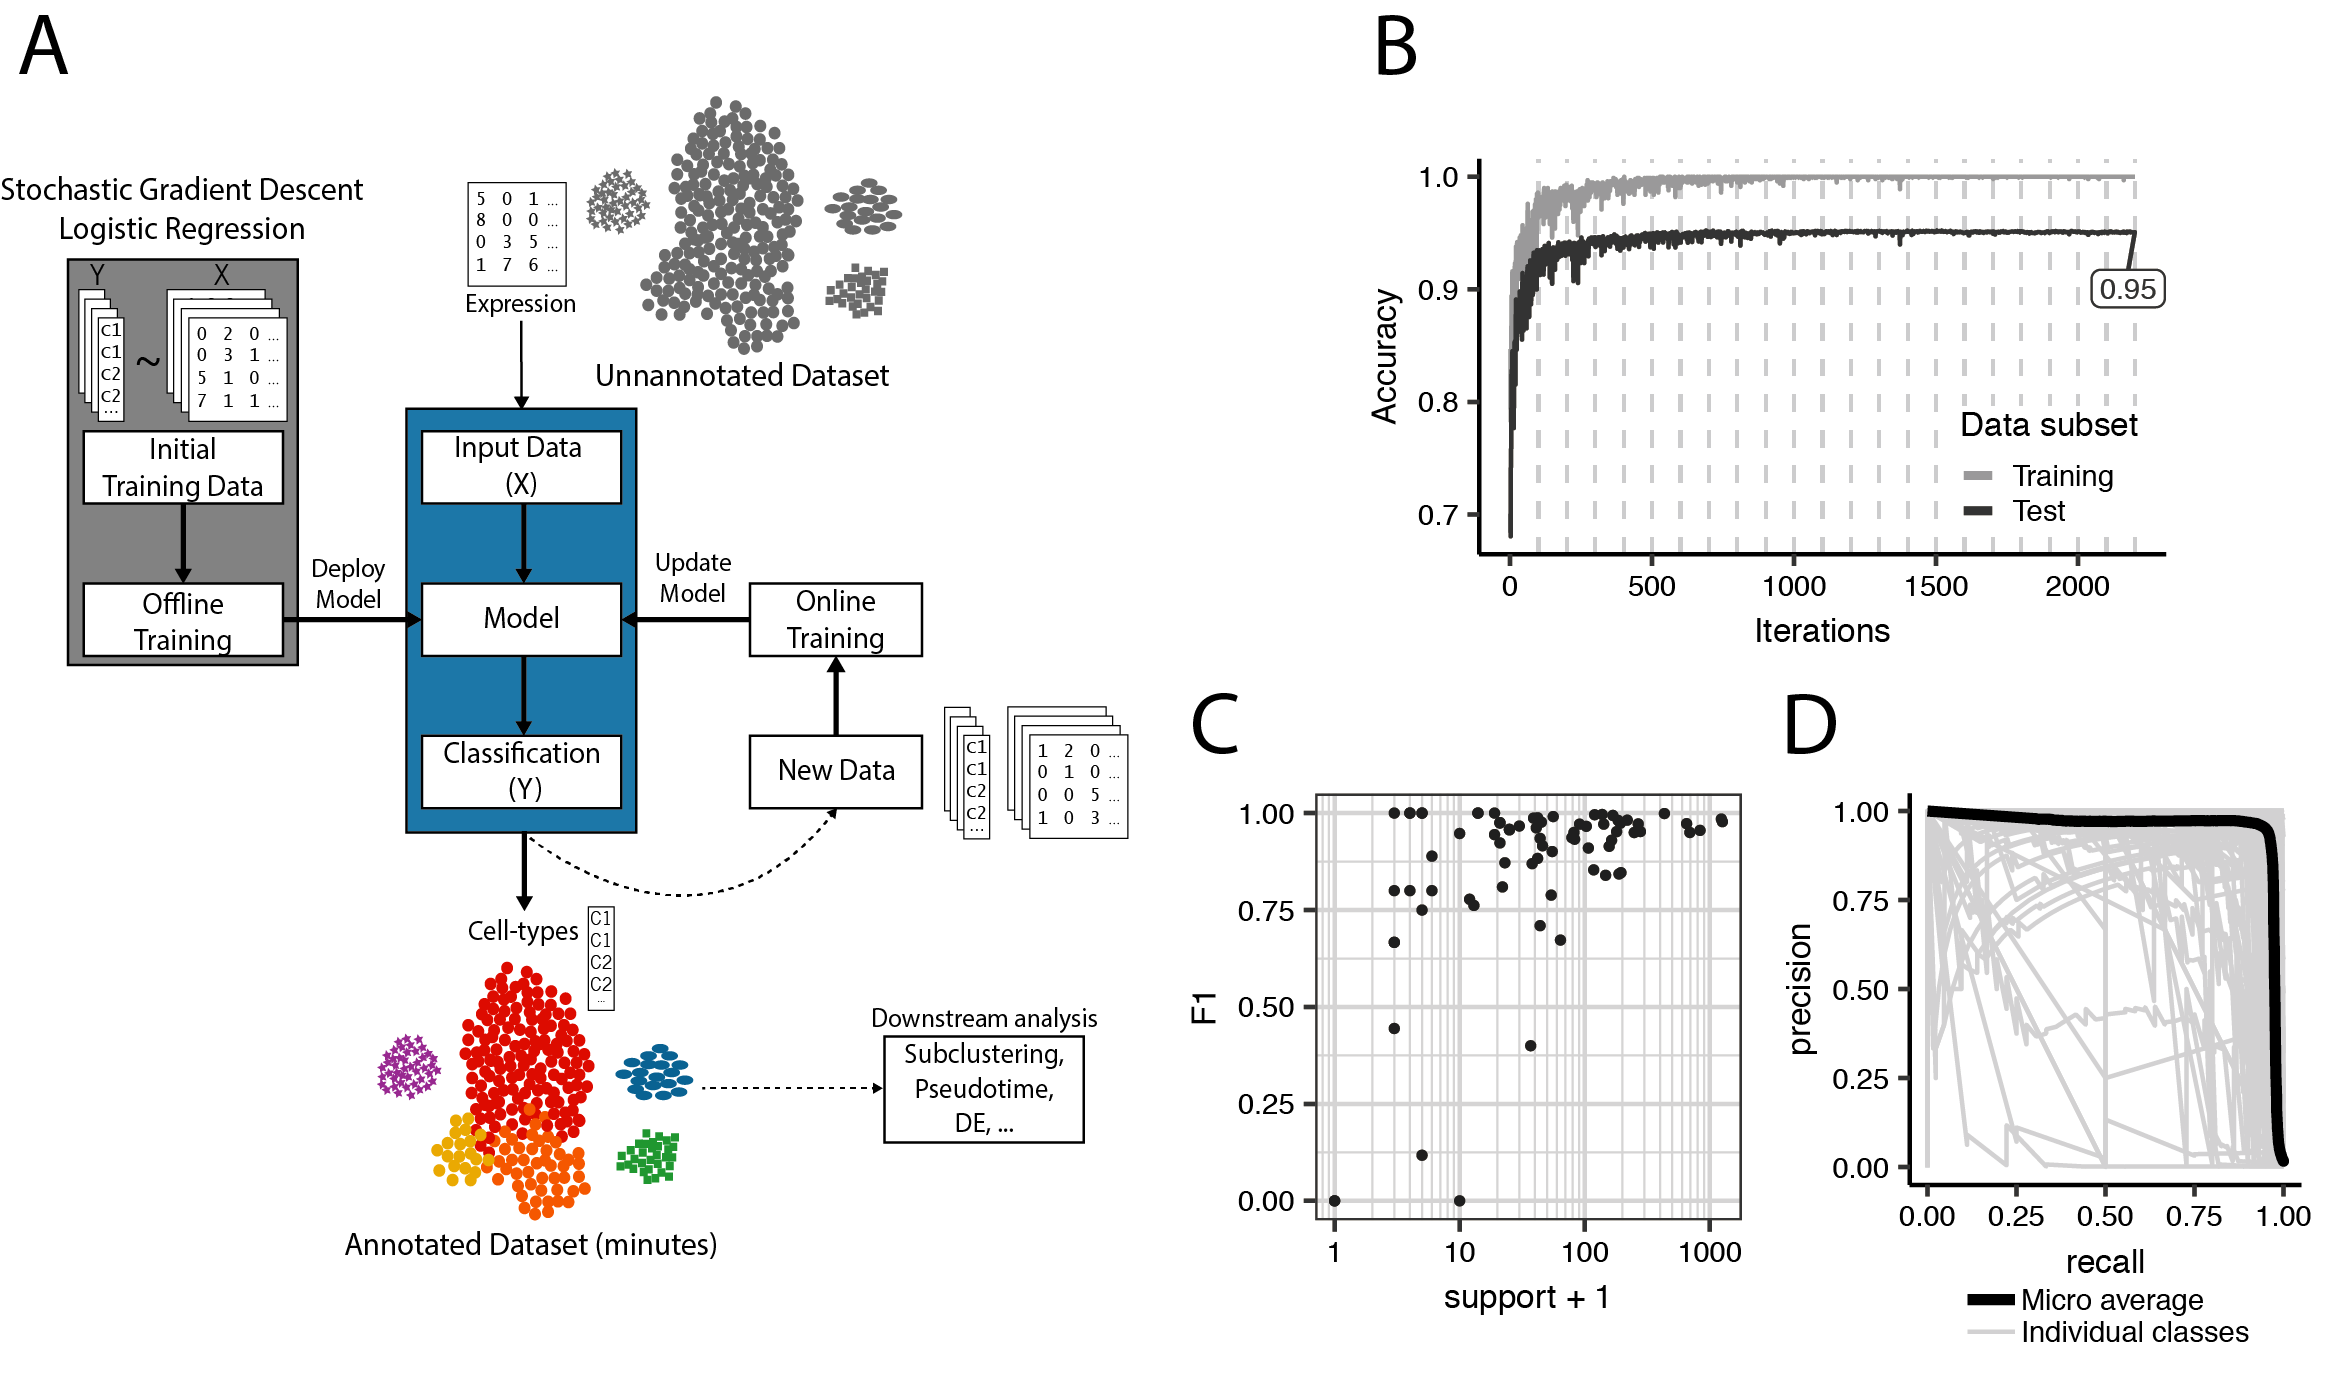
\includegraphics[width=1.0\textwidth]{Chapter3/Figs/chap3_model.png} % change word in curlies to change figure
    \caption[Model training outline and evaluation]{\textbf{Model training outline and evaluation}\newline\textbf{(A)} Model training and usage outline. A logistic regression model is trained using stochastic gradient descent. When deployed, it can provide annotations for unlabelled data, which can the be further supplied back into the model to update it. \textbf{(B)} Accuracy during model fitting for training and held-out test data, to directly predict \textit{Tabula Muris} cell type labels. Vertical dashed lines represent each training epoch. Terminal label indicated final accuracy for prediction in the test set. \textbf{(C)} F1-score for each cell type (black dots) as a function of class size (in log10 scale). \textbf{(D)} Precision-curves for each cell type (gray), and global micro average (black).}
    \label{fig:chap3_model}
\end{figure}

This methodology was first tested on the complete \textit{Tabula Muris} dataset, training the model to predict the existing cell type annotations. The model converged after fewer than 500 iterations (each iteration corresponding to a batch of 1000 cells), and resulted in a prediction accuracy of 95\% on the held-out test set (Figure~\ref{fig:chap3_model}B). Performance per class was assessed by calculating the F1 score, i.e. the harmonic mean between precision and recall for each class. A partial dependency between this score and the number of cells in a give class was observed for smaller groups (fewer than 100 cells in the test set (10\% of the total), Figure~\ref{fig:chap3_model}C, Tables~\ref{table:tab_tmmodelcells} and~\ref{table:tab_tmmodelcells2}). The strong predictive capability of the model can be further observed by plotting the precision-recall curves for each class (Figure~\ref{fig:chap3_model}D). While we again observe some classes to have a poorer performance, a micro-averaging of precision and recall of all classes (i.e. average precision and recall by calculating true positives, false positives and false negatives for each class) shows a very strong performance.

These results demonstrate the high performance of simple and intuitive logistic regression to train models capable of annotating data from various sources.


\nomenclature[z-SGD]{SGD}{Stochastic Gradient Descent}

\section{Results}
\label{section3.3}
\subsection{Training \textit{CellTypist} on the \textit{Tabula Muris} dataset}
\label{section3.3_mouse}
After integrating scRNA-seq data across tissues, as described in Sections~\ref{section3.2.1} and~\ref{section3.2.2}, the expression values can be used to unbiasedly predict cell identity by constructing a model in a similar fashion to that described in Section~\ref{section3.2.3}.

\begin{figure}[ht!]
    \centering    
    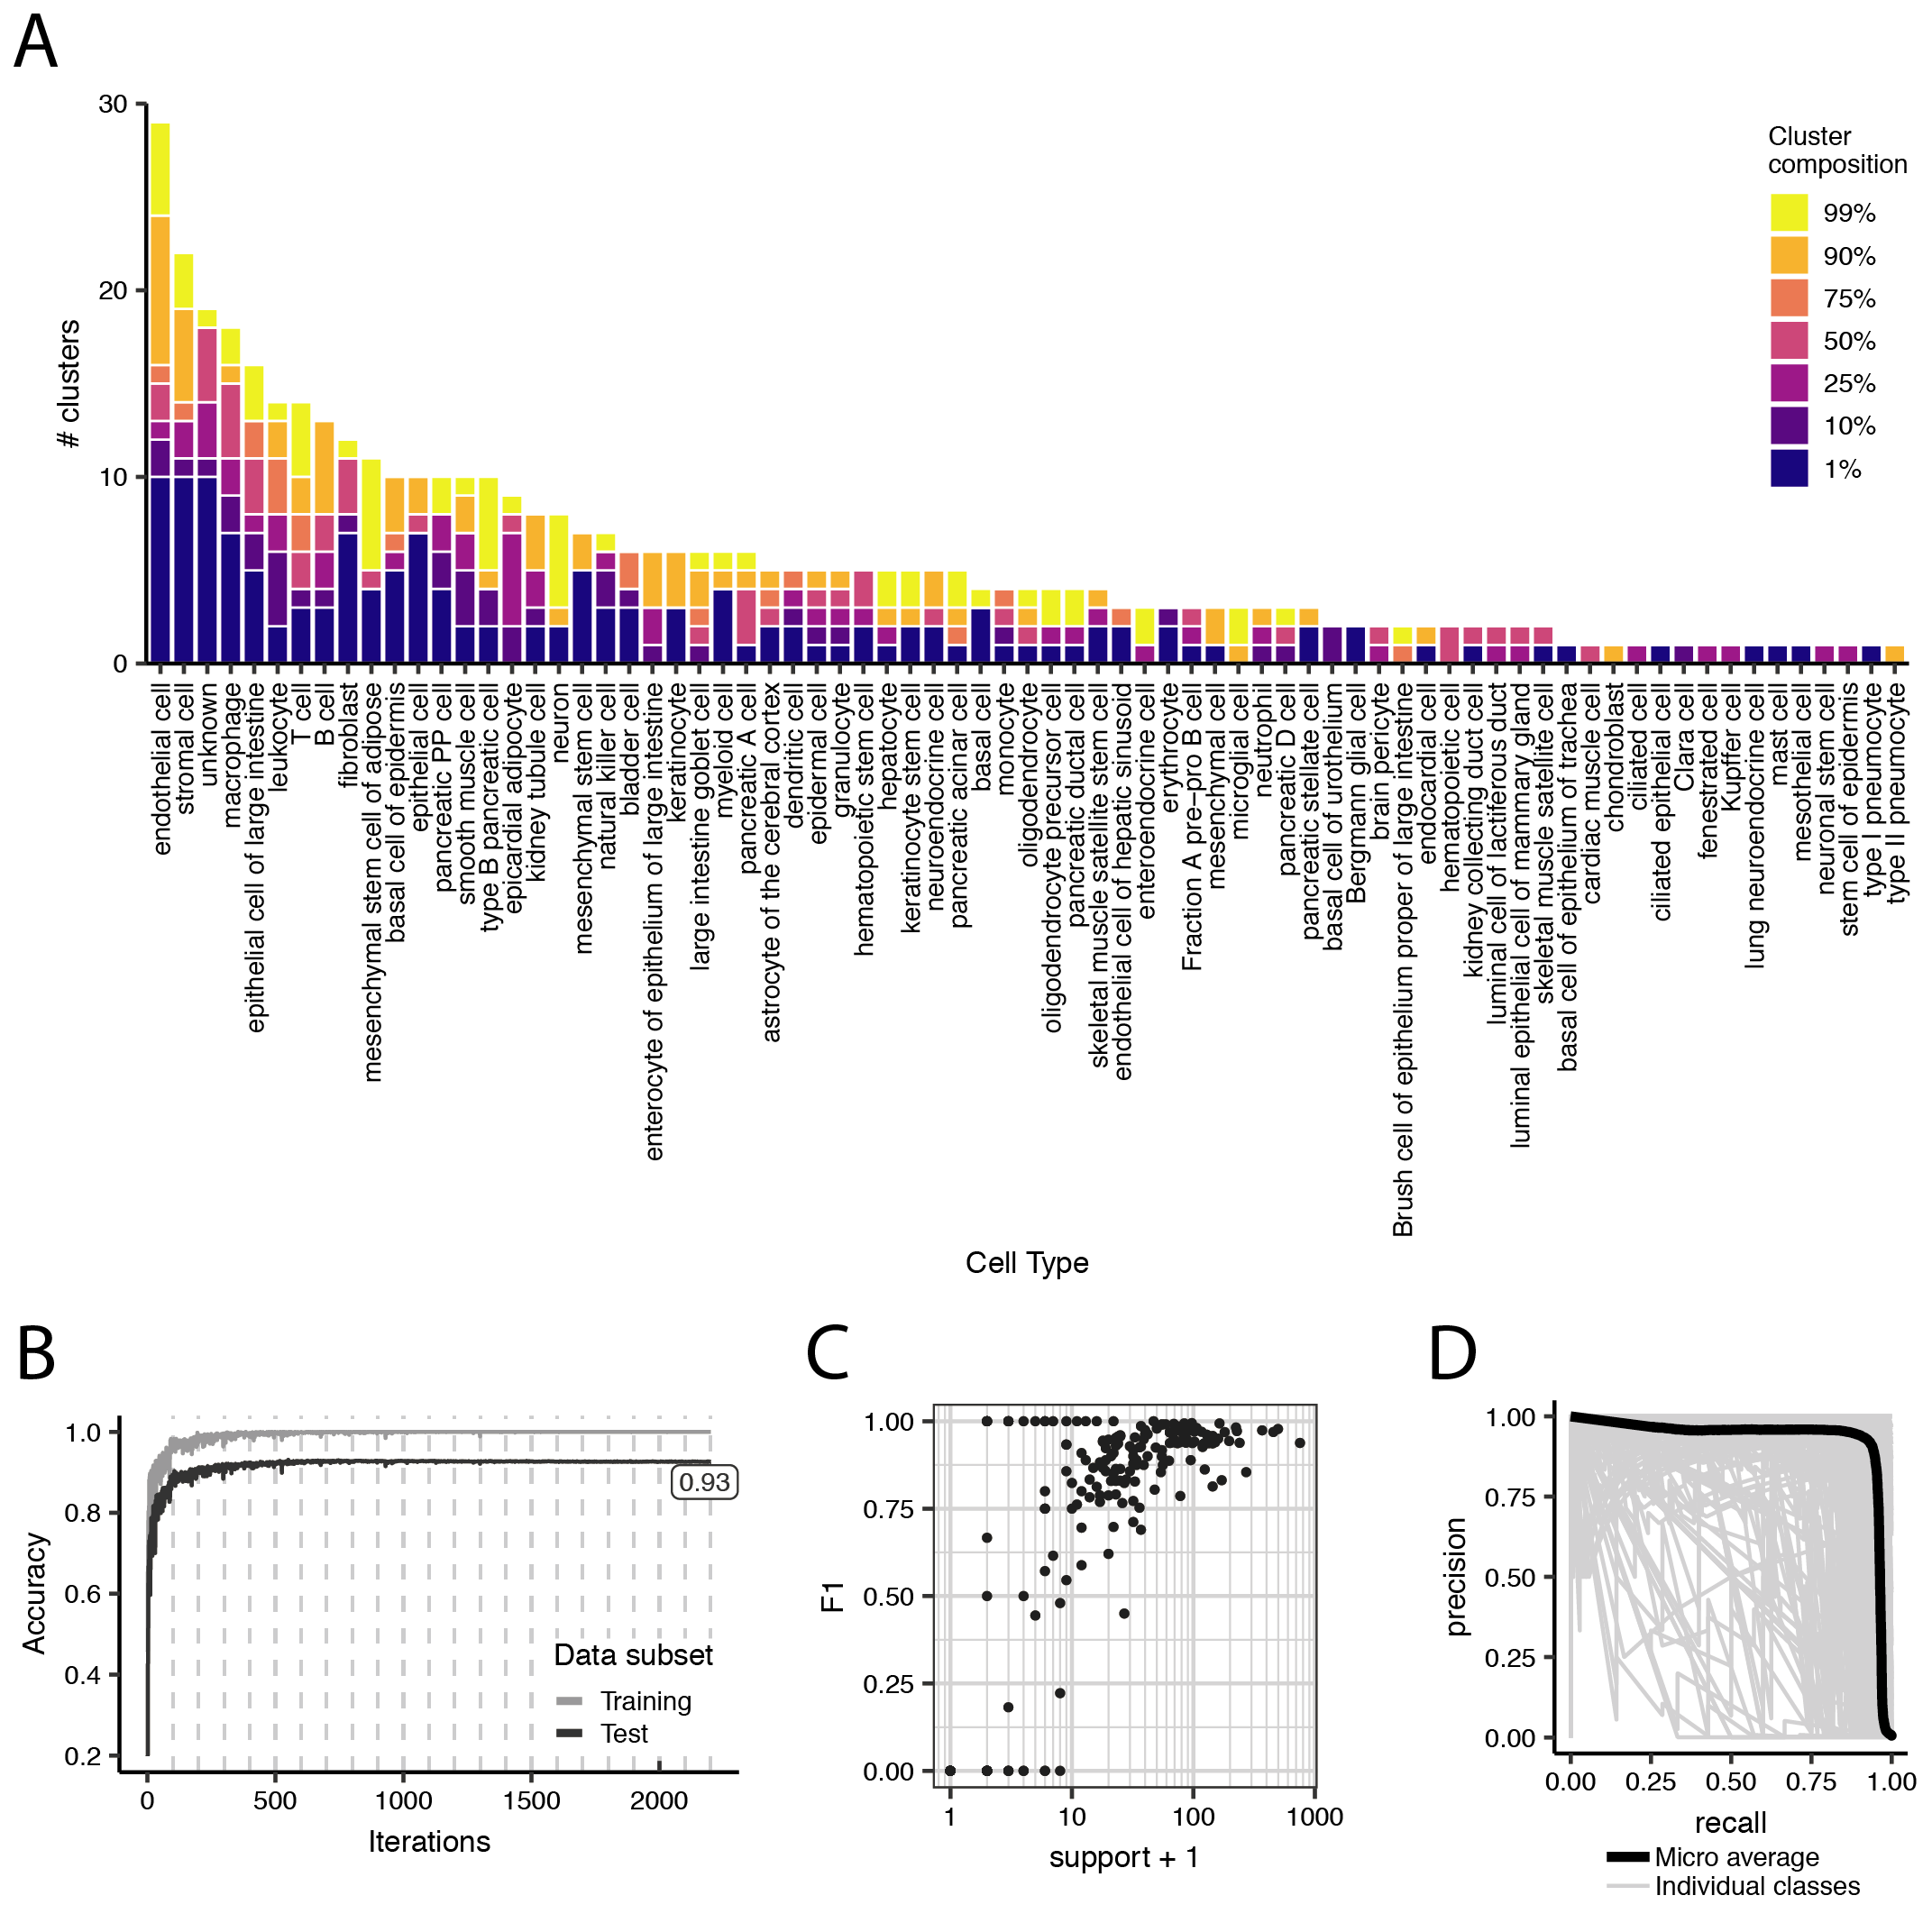
\includegraphics[scale=0.73]{Chapter3/Figs/chap3_modelcl.png} % change word in curlies to change figure
    \caption[Evaluating model trained on cross-tissue integrated clusters]{\textbf{Evaluating model trained on cross-tissue integrated clusters}\newline\textbf{(A)} Abundance of annotated cell types in cross-tissue clusters. Colours represent clusters with at least x\% of a given cell type. \textbf{(B)} Accuracy during model fitting for training and held-out test data, to predict cross-tissue integrated clusters. Vertical dashed lines represent each training epoch. Terminal label indicated final accuracy for prediction in the test set. \textbf{(C)} F1-score for each cluster label (black dots) as a function of class size (in log10 scale). \textbf{(D)} Precision-curves for each cluster (gray), and global micro average (black).}
    \label{fig:chap3_modelcl}
\end{figure}

The model training framework was thus tested using the cluster labels resulting from the merging shown in Figure~\ref{fig:chap3_combdat} (thr1 = 0.8, thr2 = 0.99). Clustering at the tissue level resulted in 222 clusters overall, compared with 139 cell type-tissue combinations. This increase was mainly registered in Pancreas (+20 clusters), Colon (+17), Fat (+11), Brain Neurons (+11) and Aorta (+9). All of these were clustered with a resolution of 0.1, and all were solely represented in Smart-seq2 derived data (Figure~\ref{fig:appB_tmcounts}). This hints at potential batch effects that were unaccounted for in the initial analysis step. Merging the clusters across tissues resulted in a final number of 198 clusters as the top result, compared to 75 unique annotated cell types, a difference that is mostly propagated for the initial large increase in the number of clusters. Nonetheless, those that were merged grouped in many cases cells with a similar phenotype (Figure~\ref{fig:chap3_combdat}).

Figure~\ref{fig:chap3_modelcl}A examines the representation of annotated cell types across all clusters, showing that a large majority of cell types are in one or more clusters where they represent at least 90\% of cells, indicating that although the number of clusters is elevated compared to expectations, most clusters are highly specific. Similarly to the cell type-based model, performance metrics globally show a fast convergence and high training accuracy (Figure~\ref{fig:chap3_modelcl}B), as well as a high per-label precision and recall (Figure~\ref{fig:chap3_modelcl}C, D), with most classes having an F1 score above 0.75. Classification performance can be seen broken down by cluster in Tables~\ref{table:tab_tmmodelclust},~\ref{table:tab_tmmodelclust1},~\ref{table:tab_tmmodelclust2}, and~\ref{table:tab_tmmodelclust3}. These again reveal the poorer performance of lowly represented clusters, many of which originating from the overclustered tissues mentioned above.


\subsection{Training \textit{CellTypist} on a collection of human data}
\label{section3.3_human}
To obtain a global, cross-tissue perspective of human cell types, we obtained a broad representation of single-cell transcriptomes by collecting several publicly available scRNA-seq datasets (Table~\ref{table:tab_humancells}). Information about tissue, scRNA-seq protocol, sampling method, and cell type annotation (when available) were obtained from the respective publications and data repositories, together with the gene expression matrices (Figure~\ref{fig:chap3_humancells}).

\begin{figure}[ht!]
    \centering    
    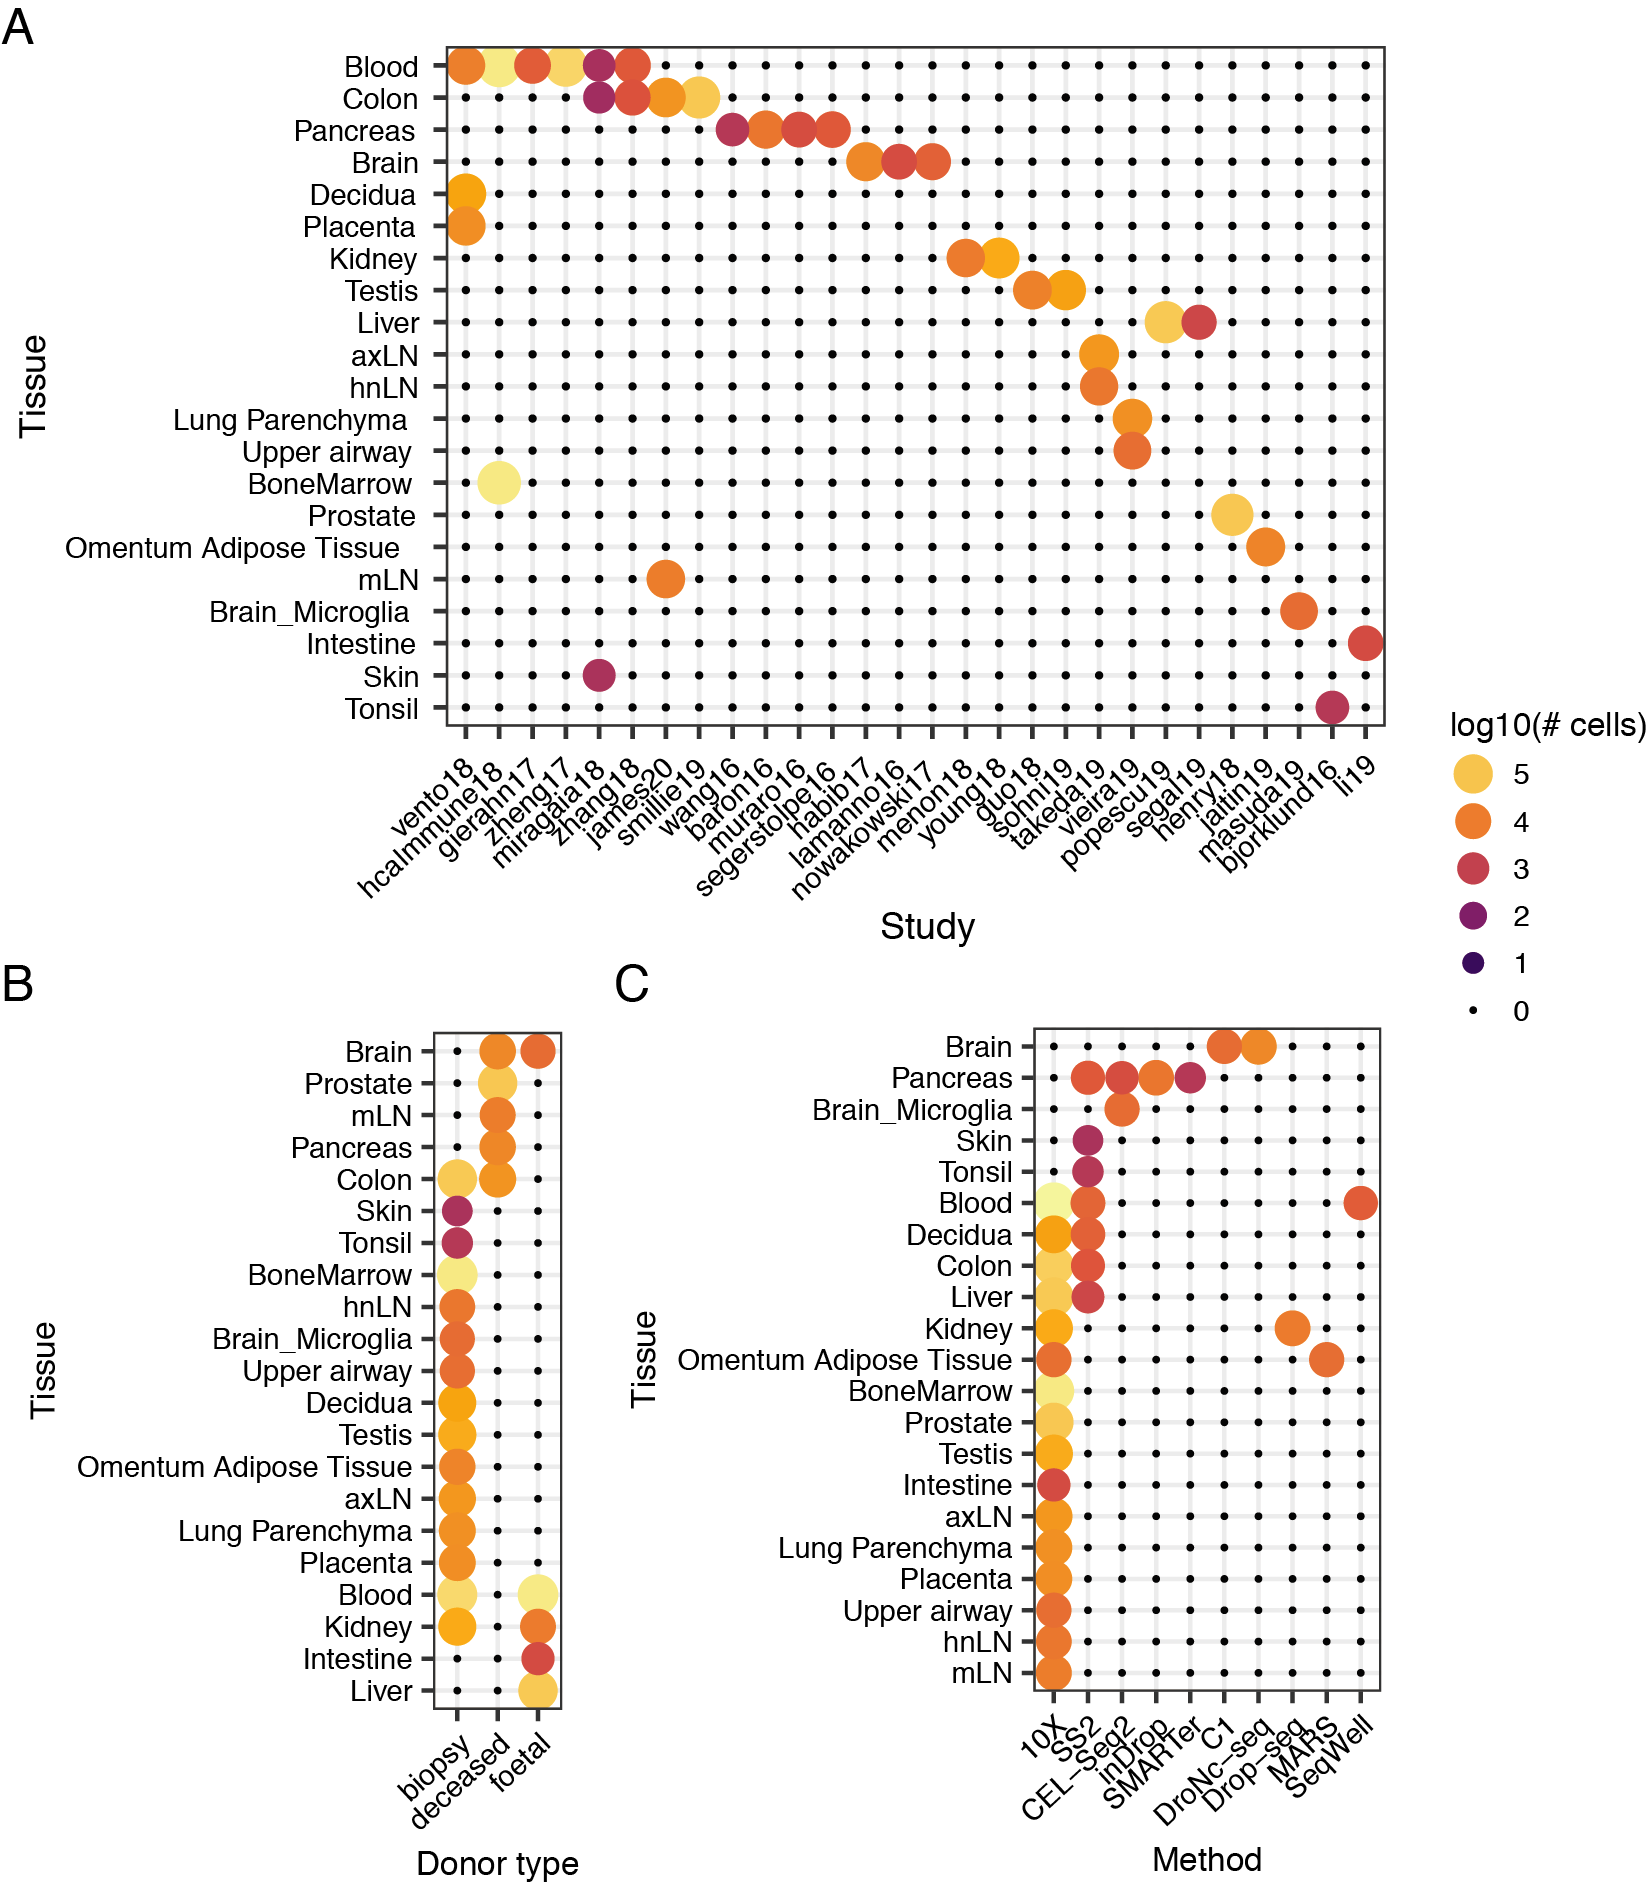
\includegraphics[width=1.0\textwidth]{Chapter3/Figs/chap4_countsHumanAtlas.png} % change word in curlies to change figure
    \caption[Cell numbers in the human dataset collection]{\textbf{Cell numbers in the human dataset collection} \newline Number of cells, in log10 scale, collected from different tissues, and distributed by publication \textbf{(A)}, type of collection \textbf{(B)}, and scRNA-seq protocol \textbf{(C)}. hnLN - head and neck lymph nodes; axLN - axilary lymph nodes; mLN - mesenteric lymph nodes.}
    \label{fig:chap3_humancells}
\end{figure}

The 28 datasets collected include 21 tissues, mostly collected from adult biopsies (Figure~\ref{fig:chap3_humancells}A and ~\ref{fig:chap3_humancells}B), and totalling close to 1.5 million cells. Various studies focus on haematopoietic-derived cells, and as such many of the sampled tissues are mostly composed of immune cells (Figure~\ref{fig:appB_ptprc}). Most cells are obtained using the droplet-based "Chromium" instrument from 10x Genomics ("10X" in Figure~\ref{fig:chap3_humancells}C), followed by the plate-based, full-length Smart-seq2 ("SS2"). Despite this imbalance in usage of different technologies, it is in agreement with what has been reported in an exhaustive curated reference of single-cell sequencing datasets~\citep{svensson_curated_2019}.

Single-cell RNA-seq expression data was collected for the publications listed in Table~\ref{table:tab_humancells}, together with cell type annotations when these were available. Information about tissue, donor type and scRNA-seq protocol were obtained from the publications.In most cases, count data was available together with the raw sequencing reads in the chosen repository. In other cases, the expression matrices deposited included log normalised data. This means that the data was normalised by the total number of reads/UMI of each cell, often followed by multiplication by a specific scaling factor (usually 10000), and finally log scaled, adding 1 to account for the zeroes present. For these datasets, data was reconverted to counts following an approach similar to that explained in \url{http://www.nxn.se/valent/2018/10/25/unscaling-scaled-counts-in-scrna-seq-data}. Briefly, given the scaling factor \textit{S}, representing the second most abundant value for each cell, and \textit{x} for each expression value, unscaled data \textit{U} was obtained by applying Formula 4.1, followed by rounding to the nearest unit to remove floating point inaccuracies.

\begin{align}
U = \frac{\mathrm{e}^{x} - 1}{S}
\end{align}

Raw count matrices were then compiled together, guaranteeing as much correspondence as possible between the diverse gene references used. All gene identifiers were mapped to the corresponding HGNC gene names, and all unique identifiers were kept. This was done to maintain the integrity of each dataset, as well as facilitate data collection and incorporation.

The \textit{CellTypist} pipeline was then applied to the complete human dataset, with parameter optimisation as described in the previous Sections. Data from the same tissues was integrated and clustered using the Leiden algorithm~\citep{traag_louvain_2019} at several resolutions. For tissues with cell type annotations, resolution was optimised using the split-join distance~\citep{dongen_performance_2000} between clusters and cell type annotation and constrained to a number of clusters at least as large as the number of cell type annotations in the largest collected dataset (Figure~\ref{fig:chap4_HA}A, see Section~\ref{section3.2.1}). This led to a total of 641 clusters in all tissues.

\begin{figure}[hb!]
    \centering    
    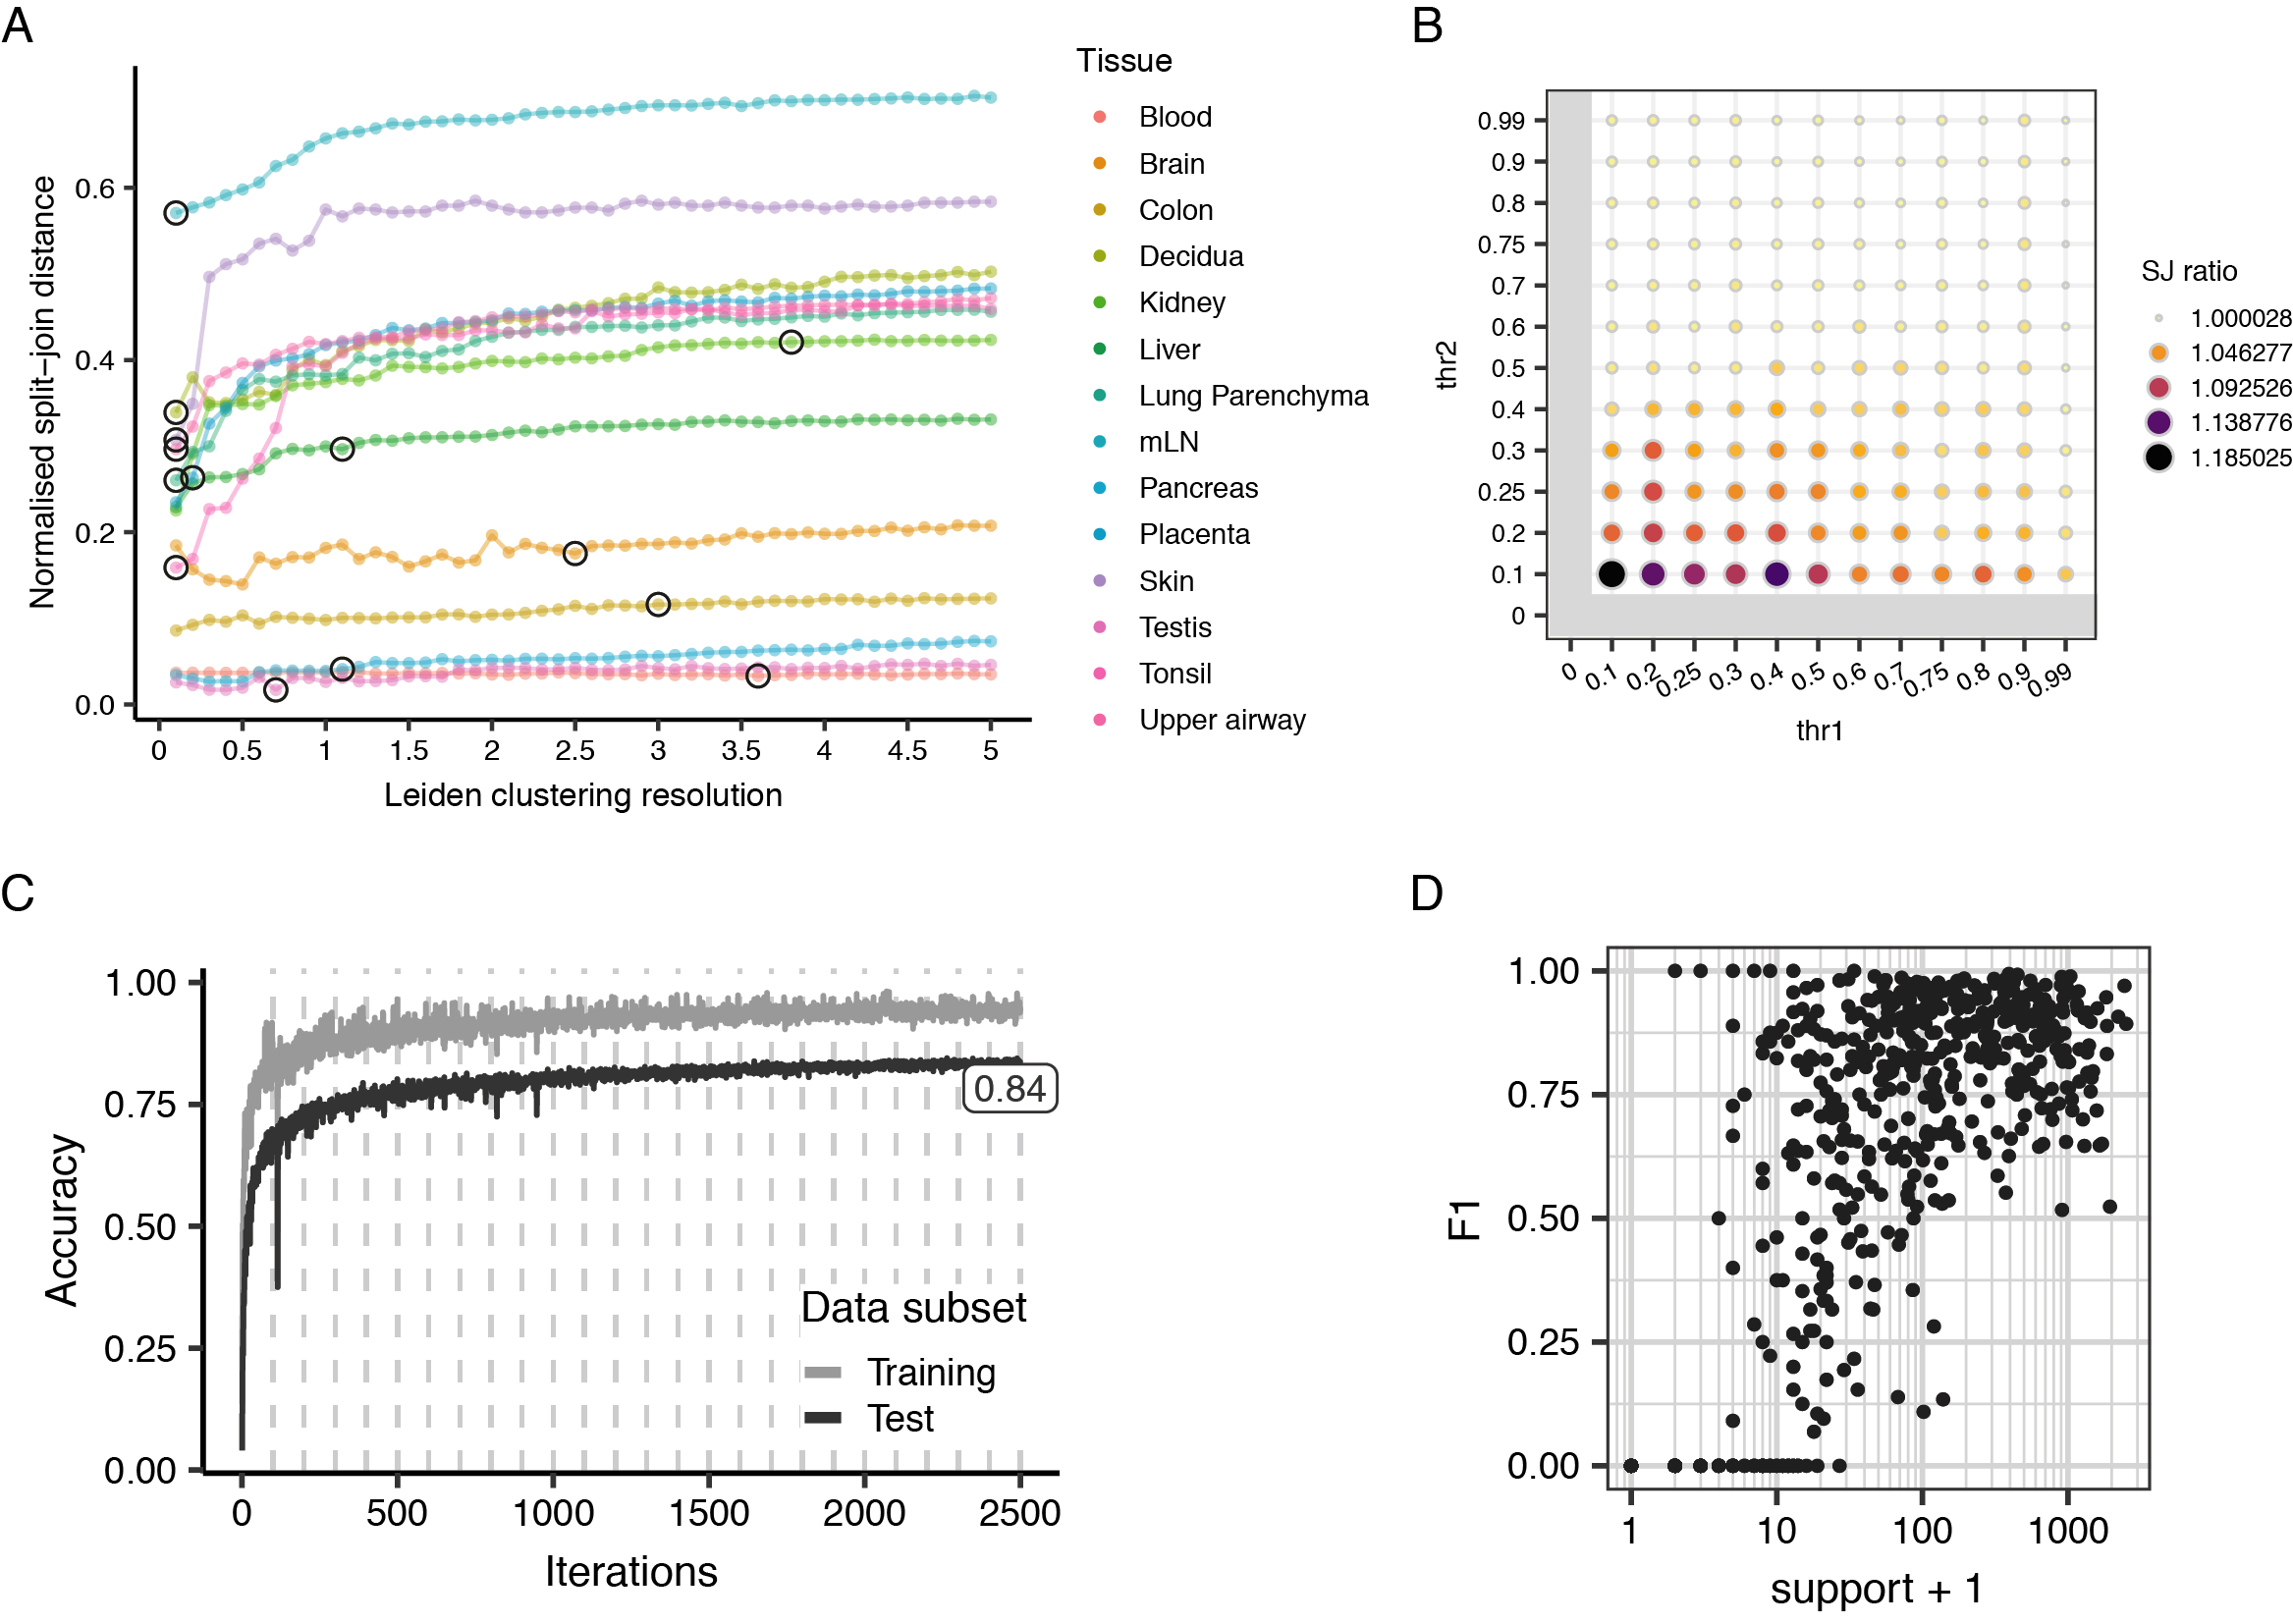
\includegraphics[width=1.0\textwidth]{Chapter3/Figs/chap4_figHA.png} % change word in curlies to change figure
    \caption[Running \textit{CellTypist} on a human scRNA-seq data collection]{\textbf{Running \textit{CellTypist} on a human scRNA-seq data collection}\newline\textbf{(A)} Per-tissue cluster optimisation, choosing the resolution that approximates existing cell type annotations. Similarity is measured with normalised split-join distance, and constrained to solutions with a number of clusters of at least as many as existing annotations in the largest collected dataset. Selected values are indicated with a black circle. \textbf{(B)} Grid of parameters tested for cross-tissue cluster merging, showing the variation of the ratio of split-join distance between merged clusters and cell type annotation, and per-tissue clusters and cell type annotation (colour and size of points). \textbf{(C)} Accuracy during model fitting for training and held-out test data, to predict cross-tissue integrated clusters obtained using thr1 = 0.99 and thr2 = 0.8 as parameters for \textit{CellTypist} (optimal value in (B)). Vertical dashed lines represent each training epoch. Terminal label indicated final accuracy for prediction in the test set. \textbf{(D)} F1-score for each cluster label (black dots) as a function of class size (in log10 scale).}
    \label{fig:chap3_HA}
\end{figure}

Following clustering, per tissue logistic regression models were trained, running for 10 epochs of a maximum of 100 iterations each. These models were used to run the cross-tissue cluster merging pipeline (Section~\ref{section3.2.2}), and a combination of parameters was chosen based on the ratio of split-join distances (merged vs annotated cell types over per tissue vs annotated cell types) (Figure~\ref{fig:chap4_HA}B, Figure~\ref{fig:appB_grids}A,B), resulting in the choice of thr1 = 0.99 and thr2 = 0.8 (627 clusters). Additionally, three other combinations were chosen for comparison: thr1 = 0.4 and thr2 = 0.99 (607 clusters), the combination with the top split-join ratio when only considering merged clusters (Figure~\ref{fig:appB_grids}C, Figure~\ref{fig:appB_moremodels}A-B); thr1 = 0.25 and thr2 = 0.25 (420 clusters), one of the combinations with the highest fraction of merged clusters (Figure~\ref{fig:appB_grids}B, Figure~\ref{fig:appB_moremodels}C-D); thr1 = 0.1 and thr2 = 0.1 (218 clusters), the combination with the highest fraction of merged clusters, as well as highest split-join fraction (Figure~\ref{fig:appB_grids}B, Figure~\ref{fig:appB_moremodels}E-F).

An example of a tissue (pancreas) with consistently annotated cell types across datasets can be seen in Figure~\ref{fig:appB_panc} with the merged clusters in the thr1 = 0.99 and thr2 = 0.8 model. We can appreciate that the pipeline, similarly to Figure~\ref{fig:chap3_combdat}C, successfully merged various similarly annotated cell types (alpha, beta, acinar, ductal, delta, gamma, epsilon, endothelial), albeit with some small "contamination" by other cell types. Other however were not so well separated, as is the case of the immune cells (t\_cell, mast, MHC class II), which were grouped together. 

The cell groupings obtained were used to train a logistic regression model using Stochastic Gradient Descent (Section~\ref{section3.2.3}). Training was done for 25 epochs of a maximum of 100 iterations each, where in each iteration 1000 cells were seen by the model. 90\% of the total data was used as a training set, and the remaining as a left out test set that was tested at every iteration (Figure~\ref{fig:chap4_HA}C, Figure~\ref{fig:appB_moremodels}). The model had a classification accuracy of 84\% on left-out test data (Figure~\ref{fig:chap3_HA}C), and the F1 statistic calculated for each label was in most cases above 0.75(Figure~\ref{fig:chap4_HA}D, Tables~\ref{table:tab_HAmodelclust} to~\ref{table:tab_HAmodelclust11}), meaning elevated precision and recall in the model, especially for clusters with more than 100 cells, as previously shown (Figure~\ref{fig:chap3_model}C, Figure~\ref{fig:chap3_modelcl}C).

Three additional models, trained using sets of clusters derived using different parameters, were also examined. These were thr1 = 0.4 and thr2 = 0.99 (Figure~\ref{fig:appB_moremodels}A-B), thr1 = 0.25 and thr2 = 0.25 (Figure~\ref{fig:appB_moremodels}C-D), and thr1 = 0.1 and thr2 = 0.1 (Figure~\ref{fig:appB_moremodels}E-F). These models show a lower performance, in particular the latter (thr1 = 0.1 and thr2 = 0.1), with a test classification accuracy of 73\%. This may be due to the excessive merging of clusters within and across tissues, thus leading to hybrid, undetermined groups of cells (Figure~\ref{fig:appC_tissrel}). Other models are more conservative in this regard, and show a better classification performance. The model using clusters obtained with thr1 = 0.25 and thr2 = 0.25 still has noticeably worse values for the split-join distance, yet also represents a more condensed cell type reference (420 clusters), without sacrificing accuracy (83\%). Lastly, the model with the parameters thr1 = 0.4 and thr2 = 0.99, in particular, is the one showing the greatest improvement in matching annotated cell types after cross-tissue merging, thus representing another possible reference model.

In sum, the collected datasets allow for the training of the \textit{CellTypist} pipeline and construct a fully interpretable human cell type reference.


\section{Discussion}
\label{section3.5}
\textit{CellTypist} has been designed as a way of systematising cell identity from expression data, and use it directly for automatic annotation. The pipeline has been designed keeping scalability in mind, fully aware that the first model represents an initial release that will be continuously updated. It is expected that the increase in data sources and available expert annotations will greatly improve the usability of the framework going forwards.

The construction of this pipeline is also subject to evolution. It has been developed with the ability to include unannotated data in a cell type reference. Existing cell type annotation is highly informative when deposited together with the expression data or the accompanying publication, although this is not always the case. Even so, the vast majority of scRNA-seq analysis pipelines rely either on Leiden~\citep{traag_louvain_2019} or Louvain~\citep{blondel_fast_2008} clustering, which are used in the per-tissue processing step and thus results in a considerable approximation between known and new labels (Figure~\ref{fig:chap3_pertiss}B). Even though the final, merged labels are to be manually curated and named, existing cell type annotations can also be made available to the end user, adding another layer of validation to the results.

The results here presented demonstrate that integration using the pipeline can correctly merge similar cell types (Figures~\ref{fig:chap3_combcl}B,C; Figure~\ref{fig:chap3_combdat}C; Figure~\ref{fig:appB_panc}C). However, these results are not perfect. The fact that, in some instances, T cells share clusters with natural killer cells, is an example that the method does not yet achieve perfect cell type separation. These two cell types have similar transcriptomes, which explains why in some reduced representations used for clustering they might appear very close. Nonetheless they are easily distinguishable by the expression of a small set of markers, and could be efficiently distinguished by a logistic regression model (Figure~\ref{fig:chap3_model}C and D). This mixing between different cell types results from both integration stages of the pipeline. Figures~\ref{fig:chap3_combdat}C and~\ref{fig:appB_panc} show that the merged clusters are composed of more than one annotated cell type, although generally containing a majority of a specific cell type, which results from the non-exact overlap between per-tissue clusters and annotated cell types. Additionally, misgrouping caused by the cross-tissue matching step (Figure~\ref{fig:chap3_combcl}B) can observed, where similar cell types can be wrongly matched (e.g. natural killer cells and T cells; smooth muscle cell and epithelial cells). These inaccuracies can be approached in various ways. 

The resolution bottleneck introduced by the first, per-tissue integration step can be potentially improved in a few ways. One possibility is to adopt a more curated approach after clustering every tissue, although this would require significantly more human input. Another option would be to rely more on data with existing annotations. One way to achieve this is by using a label propagation method that, within each integrated tissue, passes existing labels to unannotated data~\citep{barkas_joint_2019}. Alternatively, the method can instead iteratively apply the algorithm used to integrate the clusters between tissues (Figure~\ref{fig:chap3_combcl}A). In the first step this would be applied for each dataset collected to merge all existing data for each tissue, and relying on existing annotations. A second step would then be applied between tissues as shown (Figure~\ref{fig:chap3_combcl}). This guarantees that any known heterogeneity in the collected data is preserved and propagated into the final annotation, but has the disadvantage that any novel populations that would be detected by data integration can be lost, and requires the cell type labels to be thoroughly verified \textit{a priori}. Integration can also be improved by a cross-tissue batch alignment approach (using MNN~\citep{haghverdi_batch_2018} or BBKNN~\citep{polanski_bbknn:_2019}), which could potentially help with the proper overlap between cell populations, yet can be difficult to apply at scale. Lastly, an ensemble approach can also be taken by combining all the per-tissue models into a single classifier. This has the disadvantage that the pipeline will not immediately identify relationships between cell types in different tissues, yet could potentially, from the same model, match the most similar cell population and tissue.

This Chapter also demonstrated the viability of logistic regression as a methodology for cell type classification using a broad atlas as a reference (Figures~\ref{fig:chap3_model}B-D and~\ref{fig:chap3_modelcl}B-D). This is in line with previous reports~\citep{kohler_deep_2019,abdelaal_comparison_2019}, showing that cell identity classification is not improved by the use of deep learning methods, and can be accurately performed using simpler machine learning frameworks. The results also demonstrate that this method is robust enough to accommodate clusters with some mixture of cell types (which results in lower phenotypic resolution) (Figure~\ref{fig:chap3_modelcl}), and even from a broad variety of tissues and protocols (Figure~\ref{fig:chap3_HA}). However, it is important to highlight the potential biases that can arise from the collected data, since the representation of cell types in different tissues might be uneven. Differential representation of cell populations across tissues can potentially result in a bias learned by the model. As an example, if a cell type has a tissue-specific signature (that is not present in other cells from that same tissue), and this cell type is more abundantly profiled from that tissue, the gene signature learned by the model can possibly reflect, at least partially, the tissue-specific signature rather than the desired cross-tissue phenotype. While this is difficult to be considered for all cell types (due to likely tissue-specific heterogeneity and lowly abundant populations), the use of down-sampling before training or the application of a model ensemble approach could effectively mitigate this. Furthermore, imbalances in the collected data can also result in differential representation of cell populations across tissues. This is the case with the human data collection, where there is a large number of immune cells, even with some organs only being profiled at this level (Figure~\ref{fig:appB_ptprc}). This thus justified the need for an updatable model, in order to add data to incompletely profiled tissues.

The implementation of \textit{CellTypist} is also explicitly constructed such that the resulting model can be easily updated. This is due to the implementation using stochastic gradient descent, which allows for easy and direct updates to the model by running more learning iterations on novel data. This is important to maintain the reference up to date. However, it can only be done by classifying new data according to the existing labels. If the new datasets collected include cell types that are not represented in \textit{CellTypist}, then the full pipeline needs to be ran anew. Nonetheless, this allows for the database to have fast minor releases to maintain it up to date with the latest dataset publications, as well as less frequent major releases that more thoroughly integrate these datasets and revise the annotation database. \textit{CellTypist} will be available with a web interface, allowing for classifications to be ran via a web server, or, alternatively, download the models to test locally. It will include a database characterising the cell type labels present in the model. While different organisms will have different models, many of the cell types described are predicted to be present in multiple species, and can in future updates have their cross-species similarities defined and reflected in \textit{CellTypist}'s accompanying cell type compendium.

% usefulness (will be demonstrated in the next chapter)
Overall, this chapter has demonstrated that \textit{CellTypist} can organise a valuable resource for cell type annotation. Furthermore, this resource can be readily interpreted from inspection of gene coefficients for each label. In the next chapter, a practical application and interpretation of \textit{CellTypist} will be presented.